% \begin{name}
% 	{GV biên soạn: Lê Minh Cường\\ GV phản biện: Phú Thạch}
% 	{TOÁN 10-KNTT-CS}
% \end{name}
%----------------NỘI DUNG BIÊN SOẠN
\newpage
\setcounter{section}{8}
\section{Tích của một vectơ với một số}
\subsection{KIẾN THỨC TRỌNG TÂM}
\subsubsection{Tích của một vectơ với một số}
\begin{center}
	\begin{tikzpicture}[>=Stealth, line cap=round, line join=round, font=\small,scale=0.75]
		% \begin{scope}%[yshift=-160]
			% lưới + khung
			\draw[step=1, gray!30] (0,-2) grid (16,2);
			\draw[gray!55, line width=0.4pt] (0,-2) rectangle (16,2);
				\coordinate (A) at (1,0);
				\coordinate (B) at (5,0);
				\coordinate (C) at (8,1);
				\coordinate (D) at (6,1);
				\coordinate (E) at (6,-1);
				\coordinate (F) at (14,-1);

				\draw[very thick,->] (A) -- (B) node[midway, below] {$\overrightarrow a$};
				\draw[very thick,->] (C) -- (D) node[midway, above] {$\dfrac12 \overrightarrow a$};
				\draw[very thick,->]      (E) -- (F) node[midway, below] {$2\overrightarrow a$};
	\end{tikzpicture}
\end{center}
\begin{khung4}{}
	Tích của vectơ $\overrightarrow{a} \ne \overrightarrow{0}$ với số thực $k$, kí hiệu $k\overrightarrow{a}$, là một vectơ:
	\begin{itemize}
		\item có độ dài bằng $|k|\cdot \overrightarrow{a}$;
		\item cùng hướng với $\overrightarrow{a}$ khi $k\ge 0$ và ngược hướng với $\overrightarrow{a}$ khi $k<0$.
	\end{itemize}
\end{khung4}
\subsubsection{Các tính chất của phép nhân vectơ với một số}
\begin{khung4}{}
	Với hai vectơ $\overrightarrow{a}$ và $\overrightarrow{b}$ bất kì, với mọi số thực $h$ và $k$, ta có:
	\begin{enumEX}{3}
		\item $k\left (\overrightarrow{a}+\overrightarrow{b} \right )=k \overrightarrow{a}+k \overrightarrow{b}$;
		\item $(h+k) \overrightarrow{a}=h \overrightarrow{a}+k \overrightarrow{a}$;
		\item $h\left (k \overrightarrow{a}\right )=(h k) \overrightarrow{a}$;
		\item $1 \cdot \overrightarrow{a}=\overrightarrow{a}$;
		\item $-1 \cdot \overrightarrow{a}=-\overrightarrow{a}$;
		\item $k\overrightarrow{a} = \overrightarrow{0}\Leftrightarrow \hoac{&k = 0\\&\overrightarrow{a}=\overrightarrow{0}}$.
	\end{enumEX}
\end{khung4}
\begin{khung4}{}
	 \begin{itemize}
	 	\item Hai vectơ $\overrightarrow{a}$ và $\overrightarrow{b}$ ($\overrightarrow{b}$ khác $\overrightarrow{0}$) cùng phương khi và chỉ khi tồn tại số thực $k$ sao cho $\overrightarrow{a}=k \overrightarrow{b}$.
	 	\item Cho trước vectơ $\overrightarrow{a}\ne \overrightarrow{0}$. Khi đó với mọi vectơ $\overrightarrow{b}$ cùng phương với $\overrightarrow{a}$, tồn tại duy nhất số thực $x$ sao cho $\overrightarrow{b} = x\overrightarrow{a}$.
	 	\item Cho hai vectơ $\overrightarrow{a}$ và $\overrightarrow{b}$ không cùng phương. Khi đó với mọi vectơ $\overrightarrow{c}$ tồn tại duy nhất cặp số thực $(x ; y)$ sao cho $\overrightarrow{c}=x \overrightarrow{a}+y\overrightarrow{b}$.
	 \end{itemize}
\end{khung4}
\begin{khung4}{}
	\immini{Với mọi điểm M, ta có
		\begin{itemize}
		\item Nếu $I$ là trung điểm đoạn thẳng $AB$ thì $$\vec{MA}+\vec{MB}=\vec{MI}.$$
		\item Nếu $G$ là trọng tâm tam giác $ABC$ thì $$\vec{MA}+\vec{MB}+\vec{MC}=3\vec{MG}.$$
	\end{itemize}}
	{\begin{tikzpicture}[>=stealth, line cap=round, line join=round, font=\small,scale=0.7]
			\path
			(0,0) coordinate (A)
			(3.5,0) coordinate (B)
			($(A)!.5!(B)$) coordinate (I)
			(1,3) coordinate (C)
			($(C)!2/3!(I)$) coordinate (G)
			;
			\draw[thick] (A)--(B)--(C)--cycle (C)--(I);
			\foreach \d/\g in {A/-135,B/-45,I/-90,C/45,G/45} 
			{\draw (\d) circle(1.5pt) node[shift=(\g:10pt)]{$\d$};}
		\end{tikzpicture}}
\end{khung4}
%-------------------------------------------
\subsection{PHÂN LOẠI VÀ PHƯƠNG PHÁP GIẢI TOÁN}
\begin{dang}{Xác định điểm thỏa mãn đẳng thức vectơ và chứng minh}
	Dựa vào các tính chất hình học và tích của một vectơ với một số.
\end{dang}
\begin{vd}%[0H5H3-7]%[Biên soạn tài liệu dạy học bộ KNTT-CS]%[Lê Minh Cường]
	Cho hai điểm phân biệt $A,B$. Xác định điểm $M$ biết $2\overrightarrow{MA}-3\overrightarrow{MB}=\overrightarrow{0}$.
\loigiai{
	\immini
	{
	Ta có
	\begin{eqnarray*}
		&&2\overrightarrow{MA}-3\overrightarrow{MB}=\overrightarrow{0}\\
		&& 2\overrightarrow{MA}-3(\overrightarrow{MA}+\overrightarrow{AB})=\overrightarrow{0}\\
		&&-\overrightarrow{MA}-3\overrightarrow{AB}=\overrightarrow{0}\\
		&&\overrightarrow{AM}=3\overrightarrow{AB}.
	\end{eqnarray*}
	Khi đó $\overrightarrow{AM}$, $\overrightarrow{AB}$ cùng hướng và $AM=3AB$.
	}
	{
	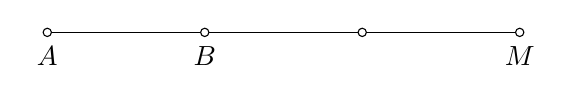
\begin{tikzpicture}[>=stealth,line join=round, line cap=round]
		\path
		(0,0) coordinate (A)
		(2,0) coordinate (B)
		(6,0) coordinate (M)
		(4,0) coordinate (H)
		;
		\draw (A)--(M);
		\foreach \x/\g in {A/-90,B/-90,M/-90}\draw[fill=white] (\x) circle (1.5pt)+(\g:3mm) node{$\x$};
		\draw[fill=white]  (H) circle (1.5pt);
	\end{tikzpicture}
	}
	}
\end{vd}\dongcham{4}

\begin{vd}%[0H5H3-7]%[Biên soạn tài liệu dạy học bộ KNTT-CS]%[Lê Minh Cường]
	Cho $\triangle ABC$, tìm $M$ thỏa $\overrightarrow{MA}-\overrightarrow{MB}+\overrightarrow{MC}=\overrightarrow{0}$.
\loigiai{
	Ta có
	\begin{eqnarray*}
		&&\overrightarrow{MA}-\overrightarrow{MB}+\overrightarrow{MC}=\overrightarrow{0}\\
		&&\overrightarrow{BA}+\overrightarrow{MC} = \overrightarrow{0}\\
		&& \overrightarrow{CM}=\overrightarrow{BA}.
	\end{eqnarray*}
	Suy ra $M$ là đỉnh thứ tư của hình bình hành $ABCM$.
	}
\end{vd}\dongcham{4}
\begin{vd}%[0H5H3-7]%[Biên soạn tài liệu dạy học bộ KNTT-CS]%[Lê Minh Cường]
	Cho $\triangle ABC$, tìm $M$ thỏa mãn  $\overrightarrow{MA}+\overrightarrow{MC}+\overrightarrow{AB}=\overrightarrow{MB}$.
\loigiai{
	Ta có
	\begin{eqnarray*}
		&&\overrightarrow{MA}+\overrightarrow{MC}+\overrightarrow{AB}=\overrightarrow{MB}\\
		&&\overrightarrow{MA}+\overrightarrow{AB}+\overrightarrow{MC}-\overrightarrow{MB}=\overrightarrow{0}\\
		&&\overrightarrow{MB}+\overrightarrow{BC}=\overrightarrow{0}\\
		&&\overrightarrow{MC}=\overrightarrow{0}.
	\end{eqnarray*}
	Suy ra $M$ trùng $C$.
	}
\end{vd}\dongcham{4}
\begin{vd}%[0H5H3-7]%[Biên soạn tài liệu dạy học bộ KNTT-CS]%[Lê Minh Cường]
	Cho hình bình hành $ABCD$. Tìm $K$ thoả mãn
	$3\overrightarrow{KA}+\overrightarrow{KB}+\overrightarrow{KC}=\overrightarrow{0}$.
\loigiai{
	\immini{
	Ta có\\
	\allowdisplaybreaks
	\begin{eqnarray*}
		&&	3\overrightarrow{KA}+\overrightarrow{KB}+\overrightarrow{KC}=\overrightarrow{0} \\
		&\Leftrightarrow& 3\overrightarrow{KC}+3\overrightarrow{CA}+\overrightarrow{KC}+\overrightarrow{CB}+\overrightarrow{KC}=\overrightarrow{0}\\
		&\Leftrightarrow& 5\overrightarrow{KC}+\overrightarrow{CA}+\overrightarrow{CB}=\overrightarrow{0}\\
		&\Leftrightarrow& 5\overrightarrow{KC}+2\overrightarrow{CN}=\overrightarrow{0} (\text{Với $N$ là trung điểm của $AB$ })\\
		&\Leftrightarrow& \overrightarrow{CK}=\dfrac{2}{5}\overrightarrow{CN}.
	\end{eqnarray*}
	}
	{
	\begin{tikzpicture}[line cap=round,line join=round]
		\coordinate[label=below:$A$] (A)at(-2,0);
		\coordinate[label=below:$B$] (B)at(1,0);
		\coordinate[label=above:$D$] (D)at(-0.3,2);
		\coordinate[label=below:$N$] (N) at ($(A)!0.5!(B)$);
		\coordinate[label=above:$C$,shift={(0:3)}] (C) at (D);
		\coordinate[label=below:$K$] (K) at ($(N)!0.6!(C)$);
		\draw (A)--(B)--(C)--(D)--cycle (N)--(C);
		\foreach \x in {A,B,C,D,N,K}
		\draw[fill=black] (\x) circle (1pt);
	\end{tikzpicture} }
	Vậy $K$ nằm trên đoạn $CN$ và cách $C$ một đoạn là $\dfrac{2}{5}CN$ với $N$ là trung điểm $AB$.
	}
\end{vd}\dongcham{7}
\begin{vd}%[0H5V3-7]%[Biên soạn tài liệu dạy học bộ KNTT-CS]%[Lê Minh Cường]
	Cho hai điểm phân biệt $A$ và $B$.
	\begin{enumerate}
		\item Hãy xác định điểm $K$ sao cho $\overrightarrow{KA}+2 \overrightarrow{KB}=\overrightarrow{0}$.
		\item Chứng minh rằng với mọi điểm $O$, ta có  $\overrightarrow{OK}=\dfrac{1}{3} \overrightarrow{OA}+\dfrac{2}{3} \overrightarrow{OB}$.
	\end{enumerate}
\loigiai{
	\immini{
	\begin{enumerate}
		\item Ta có
		\begin{eqnarray*}
			&&\overrightarrow{KA}+2 \overrightarrow{KB}=\overrightarrow{0}\\
			&&\overrightarrow{KA}+2\left(\overrightarrow{KA}+\overrightarrow{AB}\right)=\overrightarrow{0} \\
			&&3 \overrightarrow{KA}=-2 \overrightarrow{AB}\\
			&&\overrightarrow{AK}=\dfrac{2}{3} \overrightarrow{AB}
		\end{eqnarray*}
		Điểm $K$ thuộc đoạn thẳng $AB$ sao cho $AK=\dfrac{2}{3} AB$.
		\item Theo câu a) ta có
		\begin{eqnarray*}
			&&\overrightarrow{KA}+2 \overrightarrow{KB}=\overrightarrow{0}\\
			&&\overrightarrow{OA}-\overrightarrow{O K}+2\left(\overrightarrow{OB}-\overrightarrow{OK}\right)=\overrightarrow{0}\\
			&&3\overrightarrow{OK}=\overrightarrow{OA}+2 \overrightarrow{OB}\\
			&&\overrightarrow{OK}=\dfrac{1}{3} \overrightarrow{OA}+\dfrac{2}{3} \overrightarrow{OB}
		\end{eqnarray*}
	\end{enumerate}
	}{
	\begin{tikzpicture}[line join=round,line cap=round,>=stealth]
		\path
		(0,0) coordinate (A)
		(5,0) coordinate (B)
		($(A)!0.66!(B)$) coordinate (K);
		\draw[->] (A)--(B);
		\draw[->] (A)--(K);
		\foreach \p/\q in {A/90,B/90,K/90}
		\fill[black] (\p) circle (1.0pt) ($(\p)+(\q:3.0mm)$) node{$\p$};
	\end{tikzpicture}}}
\end{vd}\dongcham{10}
\begin{vd}%[0H5V3-7]%[Biên soạn tài liệu dạy học bộ KNTT-CS]%[Lê Minh Cường]
	Cho tam giác $ABC$.
	\begin{enumerate}
		\item Hãy xác định điểm $M$ để $\overrightarrow{MA}+\overrightarrow{MB}+2 \overrightarrow{MC}=\overrightarrow{0}$.
		\item Chứng minh rằng với mọi điểm $O$, ta có \ $\overrightarrow{OA}+\overrightarrow{OB}+2 \overrightarrow{OC}=4\overrightarrow{OM}$.
	\end{enumerate}
\loigiai{
	\immini{
	\begin{enumerate}
		\item Gọi $G$ là trọng tâm của tam giác $A B C$.\\ Khi đó $\overrightarrow{M A}+\overrightarrow{M B}+\overrightarrow{M C}=3 \overrightarrow{M G}$.\\
		Ta có
		\allowdisplaybreaks
		\begin{eqnarray*}
			&&\overrightarrow{M A}+\overrightarrow{M B}+2 \overrightarrow{M C}=\overrightarrow{0}\\
			& \Leftrightarrow& \overrightarrow{M A}+\overrightarrow{M B}+\overrightarrow{M C}+\overrightarrow{M C}=\overrightarrow{0}\\ &\Leftrightarrow& 3 \overrightarrow{M G}+\overrightarrow{M C}=\overrightarrow{0}\\
			& \Leftrightarrow& \overrightarrow{M C}=-3 \overrightarrow{M G}.
		\end{eqnarray*}
		Điểm $M$ thuộc đoạn thẳng $C G$ sao cho $M C=3 M G$.
		\item Theo câu a) ta có
		\begin{eqnarray*}
			&&\overrightarrow{MA}+\overrightarrow{MB}+2 \overrightarrow{MC}=\overrightarrow{0}\\
			&&\overrightarrow{OA}-\overrightarrow{OM}+\overrightarrow{OB}-\overrightarrow{OM}+2\left(\overrightarrow{OC}-\overrightarrow{OM}\right)=\overrightarrow{0}\\
			&&\overrightarrow{OA}+\overrightarrow{OB}+2 \overrightarrow{OC}=4\overrightarrow{OM}.
		\end{eqnarray*}
	\end{enumerate}
	}{\begin{tikzpicture}[line join=round, line cap=round, >=stealth]
	\path
	(0,0) coordinate (A)
	(4,0) coordinate (B)
	(2,3) coordinate (C)
	($(B)!.5!(C)$) coordinate (P)
	($(A)!.5!(C)$) coordinate (N)	($(A)!2/3!(P)$) coordinate (G)
	($(A)!0.5!(B)$) coordinate (K)
	($(C)!0.75!(G)$) coordinate (M)
	;
	\foreach \x/\y in {C/K,B/C,P/A,A/C,A/B,B/N}
	\draw (\x)--(\y);
	\foreach \x/\g in {A/180,B/0,C/90,G/180,K/-90,M/0} \fill[black] (\x) circle (1pt)+(\g:0.4) node{$\x$};
	\end{tikzpicture}}
	}
\end{vd}\dongcham{10}
\begin{dang}{Phân tích một vectơ theo hai vectơ không cùng phương}
	Vận dụng linh hoạt các tính chất.
\end{dang}
\begin{vd}%[OH5H3-5]%[Biên soạn tài liệu dạy học bộ KNTT-CS]%[Lê Minh Cường]
	Cho tam giác $ABC$. Gọi $M$ là điểm trên đoạn $BC$ sao cho $MB=2 MC$. Chứng minh rằng: $
	\overrightarrow{AM}=\dfrac{1}{3} \overrightarrow{AB}+\dfrac{2}{3} \overrightarrow{AC} .
	$
\loigiai{
	\begin{center}
		\begin{tikzpicture}[line join=round, line cap=round,thick,scale= 0.7]
			\coordinate (A) at (-1,3);
			\coordinate (B) at (-2,0);
			\coordinate (C) at (3,0);
			\coordinate (M) at ($(B)!2/3!(C)$);
			%\coordinate (G) at ($(A)!2/3!(M)$);
			\draw(A)--(B)--(C)--cycle;
			\draw(A)--(M) ;
			\foreach \i/\g in {A/90,B/-90,C/-90,M/-90}{\draw[fill=white](\i) circle (1pt) ($(\i)+(\g:3mm)$) node[scale=0.7]{$\i$};}
		\end{tikzpicture}
	\end{center}
	Ta có $\overrightarrow{BM}=\dfrac{2}{3}\overrightarrow{BC}$.\\
	$\overrightarrow{AM}=\overrightarrow{AB}+\overrightarrow{BM}=\overrightarrow{AB}+\dfrac{2}{3}\overrightarrow{BC}=\overrightarrow{AB}+\dfrac{2}{3}\left(\overrightarrow{AC}-\overrightarrow{AB}\right)=\dfrac{1}{3}\overrightarrow{AB}+\dfrac{2}{3}\overrightarrow{AC}$.
	}
\end{vd}\dongcham{6}
\begin{vd}%[OH5H3-5]%[Biên soạn tài liệu dạy học bộ KNTT-CS]%[Lê Minh Cường]
	Cho tam giác $A B C$. Gọi $K$ là điểm trên tia đối của tia $A B$ sao cho $K B=4 K A$. Hãy tính vectơ $\overrightarrow{C K}$ theo hai vectơ $\overrightarrow{BA}$ và $\overrightarrow{BC}$.
\loigiai{
	\begin{center}
		\begin{tikzpicture}[line join=round, line cap=round,thick,scale= 0.7]
			\coordinate (A) at (-1,3);
			\coordinate (B) at (-2,0);
			\coordinate (C) at (3,0);
			\coordinate (K) at ($(A)!1/-4!(B)$);
			%\coordinate (G) at ($(A)!2/3!(M)$);
			\draw(A)--(B)--(C)--cycle;
			\draw(C)--(K)--(A) ;
			\foreach \i/\g in {A/180,B/-90,C/-90,K/90}{\draw[fill=white](\i) circle (1pt) ($(\i)+(\g:3mm)$) node[scale=0.7]{$\i$};}
		\end{tikzpicture}
	\end{center}
	Ta có $\overrightarrow{BK}=\dfrac{4}{3}\overrightarrow{BA}$.\\
	$\overrightarrow{CK}=\overrightarrow{BK}-\overrightarrow{BC}=\dfrac{4}{3}\overrightarrow{BA}-\overrightarrow{BC}$.
	}
\end{vd}\dongcham{6}
\begin{vd}%[OH5H3-5]%[Biên soạn tài liệu dạy học bộ KNTT-CS]%[Lê Minh Cường]
	Cho tam giác $ABC$, gọi $I$ là điểm trên cạnh $BC$ kéo dài sao cho $IB=3 IC$.
	\begin{listEX}[1]
		\item Tính $\overrightarrow{AI}$ theo $\overrightarrow{AB}$ và $\overrightarrow{AC}$.
		\item Gọi $J$ và $K$ lần lượt là các điểm thuộc cạnh $AC$, $AB$ sao cho $JA=2 JC$ và $KB=3 KA$. Tính $\overrightarrow{JK}$ theo $\overrightarrow{AB}$ và $\overrightarrow{AC}$.
		\item Tính $\overrightarrow{BC}$ theo $\overrightarrow{AI}$ và $\overrightarrow{JK}$.
	\end{listEX}
\loigiai{
	\begin{center}
		\begin{tikzpicture}[line join=round, line cap=round,thick,scale= 0.7]
			\coordinate (A) at (-1,3);
			\coordinate (B) at (-2,0);
			\coordinate (C) at (3,0);
			\coordinate (I) at ($(B)!3/2!(C)$);
			\coordinate (J) at ($(A)!2/3!(C)$);
			\coordinate (K) at ($(A)!1/4!(B)$);
			%\coordinate (M) at ($(B)!1/2!(C)$);
			%\coordinate (G) at ($(A)!2/3!(M)$);
			\draw(A)--(B)--(C)--cycle;
			\draw(A)--(I)--(C) ;
			\draw(J)--(K) ;
			\foreach \i/\g in {A/180,B/-90,C/-90,I/0,J/90,K/180}{\draw[fill=white](\i) circle (1pt) ($(\i)+(\g:3mm)$) node[scale=0.7]{$\i$};}
		\end{tikzpicture}
	\end{center}
	\begin{listEX}[1]
		\item Ta có $\overrightarrow{BI}=\dfrac{3}{2}\overrightarrow{BC}$.\\
		$\overrightarrow{AI}=\overrightarrow{AB}+\overrightarrow{BI}=\overrightarrow{AB}+\dfrac{3}{2}\overrightarrow{BC}=\overrightarrow{AB}+\dfrac{3}{2}\left(\overrightarrow{AC}-\overrightarrow{AB}\right)=-\dfrac{1}{2}\overrightarrow{AB}+\dfrac{3}{2}\overrightarrow{AC}$ $(1)$.
		\item Ta có $\overrightarrow{AK}=\dfrac{1}{4}\overrightarrow{AB}$ và $\overrightarrow{AJ}=\dfrac{2}{3}\overrightarrow{AC}$.\\
		$\overrightarrow{JK}=\overrightarrow{AK}-\overrightarrow{AJ}=\dfrac{1}{4}\overrightarrow{AB}-\dfrac{2}{3}\overrightarrow{AC}$ $(2)$.
		\item Lấy $(1)+2\cdot(2)$ ta được $\overrightarrow{AI}+2\overrightarrow{JK}=\dfrac{1}{6}\overrightarrow{AC}\Rightarrow\overrightarrow{AC}=6\overrightarrow{AI}+12\overrightarrow{JK}$.\\
		Thay vào $(1)$ ta được $\overrightarrow{AI}=-\dfrac{1}{2}\overrightarrow{AB}+\dfrac{3}{2}\left(6\overrightarrow{AI}+12\overrightarrow{JK}\right)\Rightarrow\overrightarrow{AB}=16\overrightarrow{AI}+36\overrightarrow{JK}$.\\
		$\overrightarrow{BC}=\overrightarrow{AC}-\overrightarrow{AB}=\left(6\overrightarrow{AI}+12\overrightarrow{JK}\right)-\left(16\overrightarrow{AI}+36\overrightarrow{JK}\right)=-10\overrightarrow{AI}-24\overrightarrow{JK}$.
	\end{listEX}
	}
\end{vd}\dongcham{10}
\begin{vd}%[OH5H3-5]%[Biên soạn tài liệu dạy học bộ KNTT-CS]%[Lê Minh Cường]
	Cho $\triangle ABC$. Gọi $M$ là trung điểm của $AB$ và $N$ là điểm thỏa: $\overrightarrow{NC}=-2 \overrightarrow{NA}$. Gọi $K$ là trung điểm của $MN$.
	\begin{listEX}[1]
		\item Chứng minh rằng : $\overrightarrow{AK}=\dfrac{1}{4} \overrightarrow{AB}+\dfrac{1}{6} \overrightarrow{AC}$.
		\item Gọi $D$ là trung điểm của $BC$. Chứng minh rằng: $\overrightarrow{KD}=\dfrac{1}{4} \overrightarrow{AB}+\dfrac{1}{3} \overrightarrow{AC}$.
	\end{listEX}
\loigiai{
	\begin{center}
		\begin{tikzpicture}[line join=round, line cap=round,thick,scale= 0.7]
			\coordinate (A) at (-1,3);
			\coordinate (B) at (-2,0);
			\coordinate (C) at (3,0);
			\coordinate (M) at ($(A)!1/2!(B)$);
			\coordinate (N) at ($(A)!1/3!(C)$);
			\coordinate (K) at ($(M)!1/2!(N)$);
			\coordinate (D) at ($(B)!1/2!(C)$);
			%\coordinate (M) at ($(B)!1/2!(C)$);
			%\coordinate (G) at ($(A)!2/3!(M)$);
			\draw(A)--(B)--(C)--cycle;
			\draw(M)--(N) ;
			\draw(A)--(K)--(D) ;
			\foreach \i/\g in {A/180,B/-90,C/-90,M/180,N/0,K/-90,D/-90}{\draw[fill=white](\i) circle (1pt) ($(\i)+(\g:3mm)$) node[scale=0.7]{$\i$};}
		\end{tikzpicture}
	\end{center}
	\begin{listEX}[1]
		\item Ta có $\overrightarrow{AM}=\dfrac{1}{2}\overrightarrow{AB}$ và $\overrightarrow{AN}=\dfrac{1}{3}\overrightarrow{AC}$.\\
		$\overrightarrow{AK}=\dfrac{1}{2}\left(\overrightarrow{AM}+\overrightarrow{AN}\right)=\dfrac{1}{2}\left(\dfrac{1}{2}\overrightarrow{AB}+\dfrac{1}{3}\overrightarrow{AC}\right)=\dfrac{1}{4}\overrightarrow{AB}+\dfrac{1}{6}\overrightarrow{AC}$.
		\item $\overrightarrow{KD}=\overrightarrow{AD}-\overrightarrow{AK}=\dfrac{1}{2}\left(\overrightarrow{AB}+\overrightarrow{AC}\right)-\left(\dfrac{1}{4}\overrightarrow{AB}+\dfrac{1}{6}\overrightarrow{AC}\right)=\dfrac{1}{4}\overrightarrow{AB}+\dfrac{1}{3}\overrightarrow{AC}$.
	\end{listEX}
	}
\end{vd}\dongcham{10}
\begin{vd}%[OH5H3-5]%[Biên soạn tài liệu dạy học bộ KNTT-CS]%[Lê Minh Cường]
	Cho $\triangle ABC$ có trọng tâm $G$
	\begin{listEX}[1]
		\item Phân tích $\overrightarrow{AG}$ theo $2$ vectơ $\overrightarrow{AB}$ và $\overrightarrow{AC}$.
		\item Gọi $E$, $F$ là $2$ điểm xác định bởi các điều kiện: $\overrightarrow{EA}=2 \overrightarrow{EB}$, $3 \overrightarrow{FA}+2 \overrightarrow{FC}=\overrightarrow{0}$. Phân tích $\overrightarrow{EF}$ theo $\overrightarrow{AB}$ và $\overrightarrow{AC}$.
	\end{listEX}
\loigiai{
	\begin{center}
		\begin{tikzpicture}[line join=round, line cap=round,thick,scale= 0.7]
			\coordinate (A) at (-1,3);
			\coordinate (B) at (-2,0);
			\coordinate (C) at (3,0);
			\coordinate (E) at ($(A)!2/1!(B)$);
			\coordinate (F) at ($(A)!2/5!(C)$);
			\coordinate (M) at ($(B)!1/2!(C)$);
			\coordinate (G) at ($(A)!2/3!(M)$);
			\draw(A)--(B)--(C)--cycle;
			\draw(A)--(M) ;
			\draw(A)--(E)--(F) ;
			\foreach \i/\g in {A/180,B/180,C/-90,M/-90,G/180,E/180,F/90}{\draw[fill=white](\i) circle (1pt) ($(\i)+(\g:3mm)$) node[scale=0.7]{$\i$};}
		\end{tikzpicture}
	\end{center}
	\begin{listEX}[1]
		\item Gọi $M$ là trung điểm $BC$. Ta có $\overrightarrow{AM}=\dfrac{1}{2}\left(\overrightarrow{AB}+\overrightarrow{AC}\right)$ và $\overrightarrow{AG}=\dfrac{2}{3}\overrightarrow{AM}$. Suy ra $\overrightarrow{AG}=\dfrac{1}{3}\left(\overrightarrow{AB}+\overrightarrow{AC}\right)$.
		\item Ta có $\overrightarrow{AE}=2\overrightarrow{AB}$ và $\overrightarrow{AF}=\dfrac{2}{5}\overrightarrow{AC}$.\\
		$\overrightarrow{EF}=\overrightarrow{AF}-\overrightarrow{AE}=-2\overrightarrow{AB}+\dfrac{2}{5}\overrightarrow{AC}$.
	\end{listEX}
	}
\end{vd}\dongcham{10}
\begin{dang}{Xác định điểm thỏa mãn đẳng thức vectơ và tìm tập hợp điểm}
	\begin{itemize}
		\item {\bf Trường hợp 1:} Nếu $|\overrightarrow{MA}|=|\overrightarrow{MB}|$ với $A$ và $B$ (cố định) thì tập hợp điểm $M$ thuộc đường trung trực của đoạn thẳng $AB$.
		\item {\bf Trường hợp 2:} Nếu $|\overrightarrow{MC}|=k|\overrightarrow{AB}|$ với $A$, $B$, $C$ cho trước (cố định) thì tập hợp điểm $M$ thuộc đường tròn tâm $C$ bán kính $k\cdot AB$
		\item {\bf Trường hợp 3:}  Nếu $\overrightarrow{MA}=k\overrightarrow{BC}$  với $A$, $B$, $C$ cho trước (cố định) và \\
		Nếu $k\in\mathbb{R^+}$ thì tập hợp điểm $M$ thuộc nửa đường thẳng đi qua $A$ và song song với $BC$ theo hướng vectơ $\overrightarrow{BC}$.\\
		Nếu $k\in\mathbb{R^-}$ thì tập hợp điểm $M$ thuộc nửa đường thẳng đi qua $A$ và song song với $BC$ ngược hướng vectơ $\overrightarrow{BC}$.
	\end{itemize}
\end{dang}
\begin{vd}%[0H5V3-7]%[Biên soạn tài liệu dạy học bộ KNTT-CS]%[Lê Minh Cường]
	Cho $\triangle ABC$. Tìm tập hợp điểm $M$ thỏa mãn điều kiện:
	\begin{listEX}[1]
		\item $\left|\overrightarrow{MA}+\overrightarrow{MB}\right|=\left|\overrightarrow{MA}+\overrightarrow{MC}\right|$;
		\item $|\overrightarrow{MA}+\overrightarrow{MB}|=|\overrightarrow{MA}-\overrightarrow{MC}|$;
		\item $3\left|\overrightarrow{MA}+\overrightarrow{MB}\right|=2\left|\overrightarrow{MA}+\overrightarrow{MB}+\overrightarrow{MC}\right|$.
	\end{listEX}
\loigiai{
	\begin{enumerate}
		\item Gọi $I$, $K$ lần lượt là trung điểm của $AB$, $AC$.\\
		Ta có $\left|\overrightarrow{MA}+\overrightarrow{MB}\right|=\left[\overrightarrow{MA}+\overrightarrow{MC}\right]$.\\
		Khi đó $2\left|\overrightarrow{MI}\right|=2\left|\overrightarrow{MK}\right|$.\\
		Vậy $|\overrightarrow{MI}|=|\overrightarrow{MK}|$, hay tập hợp điểm $M$ thuộc trung trực của $IK$.
		\item Gọi $I$ là trung điểm $AB$, khi đó
		$|\overrightarrow{MA}+\overrightarrow{MB}|=|\overrightarrow{MA}-\overrightarrow{MC}|$ $\Rightarrow 2|\overrightarrow{MI}|=|\overrightarrow{CA}|$ $\Rightarrow |\overrightarrow{MI}|=\dfrac{1}{2} AC$. \\
		Vậy tập hợp điểm $M$ thuộc đường tròn tâm $I$ bán kính $\dfrac{AC}{2}$.
		\item Gọi $G$ là trọng tâm tam giác $ABC$, $I$ là trung điểm $AB$, ta có
		\begin{eqnarray*}
			&&3\left|\overrightarrow{MA}+\overrightarrow{MB}\right|=2\left|\overrightarrow{MA}+\overrightarrow{MB}+\overrightarrow{MC}\right|\\
			&&6\left|\overrightarrow{MI}\right|=6\left|\overrightarrow{MG}\right|\\
			&&\left|\overrightarrow{MI}\right|=\left|\overrightarrow{MG}\right|.
		\end{eqnarray*}
		Vậy tập hợp $M$ thuộc đường trung trực của $IG$.
	\end{enumerate}
	}
\end{vd}\dongcham{10}
\begin{vd}%[0H5V3-7]%[Biên soạn tài liệu dạy học bộ KNTT-CS]%[Lê Minh Cường]
	Cho tam giác $ABC$, gọi $D$ là trung điểm $BC$, gọi $E$ là trung điểm $AD$, gọi $I$ là trung điểm $CE$.
	\begin{enumerate}
		\item Biểu diễn $\overrightarrow{AI}$, $\overrightarrow{DI}$ theo hai vectơ $\overrightarrow{AC}$, $\overrightarrow{AB}$.
		\item Tìm tập hợp điểm $M$ sao cho $2\left|\overrightarrow{MA} + \overrightarrow{ME} + \overrightarrow{MC}\right|=3\left|\overrightarrow{MD} + \overrightarrow{MA}\right|$.
	\end{enumerate}
\loigiai{
	\begin{tikzpicture}[>=stealth]
		\coordinate[label = left:$B$] (B) at (0,0);
		\coordinate[label = right:$C$] (C) at ($(B)+(8,0)$);
		\coordinate[label = above:$A$, shift=(70:6cm)] (A) at (B);
		\coordinate[label = below:$D$] (D) at ($(B)!1/2!(C)$);
		\coordinate[label = below  left:$E$] (E) at ($(A)!1/2!(D)$); % Định nghĩa điểm M thỏa mãn \vt{AM}=1/2*\vt{AB}
		\coordinate[label = below:$I$] (I) at ($(E)!1/2!(C)$);
		%\coordinate[label = left:$I$] (I) at ($(A)!2/3!(B)$);
		\coordinate[label =left:$J$] (J) at ($(A)!2/3!(I)$);
		\draw (A)--(B)--(C)--cycle;
		\foreach \x in {A,B,C,D,E,I,J} \fill[black] (\x) circle (1.5pt);
		\draw(A)--(D)--(E);
		\draw(C)--(I)--(E);
		\draw[thick] (A)--(I);
		\draw[thick] (D)--(I);
	\end{tikzpicture}
	\begin{enumerate}
		\item Ta có
		\begin{eqnarray*}
			2\overrightarrow{AI}&=&\overrightarrow{AE}+\overrightarrow{AC}\\
			&=&\dfrac{1}{2}\overrightarrow{AD}+\overrightarrow{AC}\\
			&=&\dfrac{1}{4}\left(\overrightarrow{AB}+\overrightarrow{AC} \right) +\overrightarrow{AC}\\
			&=&\dfrac{1}{4}\overrightarrow{AB}+\dfrac{5}{4}\overrightarrow{AC}
		\end{eqnarray*}
		Suy ra $\overrightarrow{AI}=\dfrac{1}{8}\overrightarrow{AB}+\dfrac{5}{8}\overrightarrow{AC}$.\\
		Mặt khác,
		\begin{eqnarray*}
			\overrightarrow{DI}&=&\overrightarrow{AI}-\overrightarrow{AD}\\
			&=&\dfrac{1}{8}\overrightarrow{AB}+\dfrac{5}{8}\overrightarrow{AC}-\dfrac{1}{2}\left(\overrightarrow{AB}+\overrightarrow{AC} \right)\\
			&=&-\dfrac{3}{8}\overrightarrow{AB}+\dfrac{1}{8}\overrightarrow{AC}
		\end{eqnarray*}
		\item Gọi $J$ là trọng tâm $\bigtriangleup AEC$, ta có,  $\heva{&\overrightarrow{MA} + \overrightarrow{ME} + \overrightarrow{MC}=3\overrightarrow{MJ}+\overrightarrow{JA} + \overrightarrow{JE} + \overrightarrow{JC}=3\overrightarrow{MJ}\\&\overrightarrow{MD} + \overrightarrow{MA}=2\overrightarrow{ME} + \overrightarrow{EA}+ \overrightarrow{ED}=2\overrightarrow{ME}}$. \\
		Suy ra $\heva{&2\left|\overrightarrow{MA} + \overrightarrow{ME} + \overrightarrow{MC}\right|=6\left|\overrightarrow{MJ}=6MJ\right|\\&3\left|\overrightarrow{MD} + \overrightarrow{MA}\right|=6\left|\overrightarrow{ME}\right|=6ME.}$\\
		Từ giả thiết ta được $MJ=ME$. \\
		Vậy tập hợp điểm $M$ là đường trung trực của đoạn thẳng $EJ$.
	\end{enumerate}}
\end{vd}\dongcham{12}
\begin{vd}%[0H5C3-7]%[Biên soạn tài liệu dạy học bộ KNTT-CS]%[Lê Minh Cường]
	Cho hình vuông $ABCD$ cạnh $2a$ tâm $O$. Hãy tìm tập hợp điểm $M$ thỏa mãn điều kiện
	\[ \left|\overrightarrow{MA}+\overrightarrow{MB}+\overrightarrow{MC}+\overrightarrow{MD}\right|=\left|\overrightarrow{AB}-\overrightarrow{AD}\right|. \]
\loigiai{
	\immini
	{
	Ta có $\overrightarrow{AB}-\overrightarrow{AD}=\overrightarrow{DB}$ và $\overrightarrow{MA}+\overrightarrow{MB}+\overrightarrow{MC}+\overrightarrow{MD}=4\overrightarrow{MO}$.\\
	Do đó, ta có $4MO=DB$ hay $OM=\dfrac{1}{4}BD=\dfrac{1}{4}\cdot 2\sqrt{2} a=\dfrac{\sqrt{2}}{2}\cdot a$.\\
	Vậy tập hợp điểm $M$ là đường tròn tâm $O$, bán kính $\dfrac{\sqrt{2}}{2}\cdot a$.
	}
	{
	\begin{tikzpicture}[line join = round, line cap = round,>=stealth]
		\path
		(0,0) coordinate (A)
		(4,0) coordinate (B)
		(0,-4) coordinate (D)
		($(B)+(D)-(A)$) coordinate (C)
		($(A)!.5!(C)$) coordinate (O)
		($(O)!.5!(B)$) coordinate (I)
		;
		\draw let\p1=($(O)-(I)$) in (O) circle({veclen(\x1,\y1)});
		\draw (A) rectangle (C);
		\draw (B)--(D);
		\foreach \x/\g in {A/90,B/90,C/-90,D/-90,O/-90}\draw[fill=white] (\x) circle (1pt)+(\g:3mm) node{$\x$};
	\end{tikzpicture}
	}
	}
\end{vd}\dongcham{12}
\begin{vd}%[0H5C3-7]%[Biên soạn tài liệu dạy học bộ KNTT-CS]%[Lê Minh Cường]
	Cho hình thoi $ABCD$ cố định có tâm $O$, cạnh bằng $a$ và góc $\widehat{ABC}=60^{\circ}$. Gọi $I$ là trung điểm của đoạn $DO$. Tìm tập hợp điểm $M$ thỏa mãn điều kiện $\left|\overrightarrow{MA}+\overrightarrow{MB}+\overrightarrow{MC}+\overrightarrow{MD}\right|=4\left|\overrightarrow{MA}+\overrightarrow{ID}\right|$.
\loigiai{
	\immini
	{
	Ta có $\overrightarrow{MA}+\overrightarrow{MB}+\overrightarrow{MC}+\overrightarrow{MD}=4\overrightarrow{MO}$.\\
	Kẻ $\overrightarrow{AE}=\overrightarrow{ID}$, khi đó $\overrightarrow{MA}+\overrightarrow{ID}=\overrightarrow{MA}+\overrightarrow{AE}=\overrightarrow{ME}$.\\
	Khi đó
	\begin{eqnarray*}
		&&\left|\overrightarrow{MA}+\overrightarrow{MB}+\overrightarrow{MC}+\overrightarrow{MD}\right|=4\left|\overrightarrow{MA}+\overrightarrow{ID}\right|\\
		&&4MO=4ME\\
		&&MO=ME
	\end{eqnarray*}
	Vậy tập hợp điểm $M$ nằm trên đường trung trực của đoạn thẳng $OE$.
	}
	{
	\begin{tikzpicture}[line join = round, line cap = round
		,declare function={
		gA=120;
		canh=3;
		}]
		\path
		(0,0) coordinate (A)
		({gA/2}:canh) coordinate (B)
		({-gA/2}:canh) coordinate (D)
		($(B)+(D)-(A)$) coordinate (C)
		($(A)!.5!(C)$) coordinate (O)
		($(D)!.5!(O)$) coordinate (I)
		($(D)+(A)-(I)$) coordinate (E)
		($(E)!0.5!(O)$) coordinate (J)
		;
		\draw (A) --(B)--(C)--(D)--cycle--(C) (B)--(D);
		\draw (O)--(E);
		\draw[->] (A)--(E);
		\foreach \x/\g in {A/180,B/90,C/0,D/-90,O/-45,E/180,I/20}\draw[fill=white] (\x) circle (1pt)+(\g:3mm) node{$\x$};
		\draw[line width=1.5pt,red] ($(J)!2!90:(O)$)--($(J)!2!-90:(O)$);
	\end{tikzpicture}
	}
	}
\end{vd}\dongcham{12}
\begin{vd}%[0H5C3-7]%[Biên soạn tài liệu dạy học bộ KNTT-CS]%[Lê Minh Cường]
	Cho hình vuông $ABCD$ cạnh $a$. Gọi $P, Q$ là các điểm thỏa mãn $\overrightarrow{BP}=\overrightarrow{BC}-2 \overrightarrow{AB}$ và $\overrightarrow{CQ}=-\dfrac{1}{2} \overrightarrow{AC}-\overrightarrow{BC}$.
	\begin{listEX}[1]
		\item Chứng minh ba điểm $A, P, Q$ thẳng hàng.
		\item Tìm tập hợp điểm $M$ thỏa mãn $\left|\overrightarrow{MA}+\overrightarrow{MB}+\overrightarrow{MC}+\overrightarrow{MD}\right|=4a\sqrt{3}$.
	\end{listEX}
\loigiai{
	\begin{listEX}[1]
		\item Ta có $\overrightarrow{AP}=\overrightarrow{AB}+\overrightarrow{BP}=\overrightarrow{AB}+\overrightarrow{BC}-2 \overrightarrow{AB}=\overrightarrow{BC}-\overrightarrow{AB}=\overrightarrow{BC}+ \overrightarrow{BA}= \overrightarrow{BD}$.\\
		Bên cạnh đó, $\overrightarrow{AQ}=\overrightarrow{AC}+\overrightarrow{CQ}=\overrightarrow{AC}-\dfrac{1}{2} \overrightarrow{AC}-\overrightarrow{BC}=\dfrac{1}{2} \overrightarrow{AC}+\overrightarrow{CB}=\overrightarrow{OC}+\overrightarrow{CB}=\overrightarrow{OB}$.\\
		Vậy $\overrightarrow{AP}=-2\overrightarrow{AQ}$, do đó $A,P,Q$ thẳng hàng.
		\item Ta có $\overrightarrow{MA}+\overrightarrow{MB}+\overrightarrow{MC}+\overrightarrow{MD}=4\overrightarrow{MO}$.\\
		Do đó $\left|\overrightarrow{MA}+\overrightarrow{MB}+\overrightarrow{MC}+\overrightarrow{MD}\right|=4a\sqrt{3}\Leftrightarrow 4MO=4a\sqrt{3}\Leftrightarrow OM=a\sqrt{3}$.\\
		Vậy tập hợp điểm $M$ là đường tròn tâm $O$, bán kính $a\sqrt{3}$.
	\end{listEX}
	}
\end{vd}\dongcham{10}
\begin{vd}%[0H5C3-7]%[Biên soạn tài liệu dạy học bộ KNTT-CS]%[Lê Minh Cường]
	Cho hình vuông $ABCD$ cạnh bằng $a$ và có tâm $O$. Gọi $N \in CD$ sao cho $CD=2CN$.
	\begin{listEX}
		\item Biểu diễn $\overrightarrow{AN}$ theo $\overrightarrow{AB}, \overrightarrow{AC}$.
		\item Tìm tập hợp điểm $M$ thỏa mãn $\left|\overrightarrow{MA}+\overrightarrow{MB}+\overrightarrow{MC}+\overrightarrow{MD}\right|=4AB$.
	\end{listEX}
\loigiai{
	\immini
	{
	\begin{listEX}[1]
		\item Ta có
		\begin{eqnarray*}
			\overrightarrow{AN}&=&\overrightarrow{AD}+\overrightarrow{DN}\\
			&=&\overrightarrow{AC}+\overrightarrow{CD}+\dfrac{1}{2}\overrightarrow{AB}\\
			&=&\overrightarrow{AC}-\overrightarrow{AB}+\dfrac{1}{2}\overrightarrow{AB}\\
			&=&\overrightarrow{AC}-\dfrac{1}{2}\overrightarrow{AB}.
		\end{eqnarray*}
		\item Ta có $\overrightarrow{MA}+\overrightarrow{MB}+\overrightarrow{MC}+\overrightarrow{MD}=4\overrightarrow{MO}$.\\
		Do đó
		\begin{eqnarray*}
			&&\left|\overrightarrow{MA}+\overrightarrow{MB}+\overrightarrow{MC}+\overrightarrow{MD}\right|=4AB\\
			&&4MO=4AB\\
			&&OM=AB=a\\
			&&OM=a.
		\end{eqnarray*}
		Vậy tập hợp điểm $M$ là đường tròn tâm $O$, bán kính $a$.
	\end{listEX}
	}
	{
	\begin{tikzpicture}[line join = round, line cap = round,>=stealth,
		declare function={a=4;}
		]
		\path
		(0,0) coordinate (A)
		(a,0) coordinate (B)
		(0,-a) coordinate (D)
		($(B)+(D)-(A)$) coordinate (C)
		($(A)!.5!(C)$) coordinate (O)
		($(D)!.5!(C)$) coordinate (N)
		;
		\pgfresetboundingbox
		\draw (A) rectangle (C);
		\draw[->] (A)--(N) (A)--(C);
		\foreach \x/\g in {A/90,B/90,C/-90,D/-90,O/70,N/-90}\draw[fill=white] (\x) circle (1pt)+(\g:3mm) node{$\x$};
	\end{tikzpicture}
	}
	}
\end{vd}\dongcham{12}
\begin{dang}{Các dạng toán thực tế}
	Vận dụng linh hoạt các kiến thức về vectơ.
\end{dang}
\begin{vd}%[0H5V3-9]%[Biên soạn tài liệu dạy học bộ KNTT-CS]%[Lê Minh Cường]
	Cho $3$ lực $\overrightarrow{F_1}$, $\overrightarrow{F_2}$, $\overrightarrow{F_3}$ cùng tác động vào một chất điểm $M$. Biết các độ lớn $F_1=7N$, $F_2=4N$, $F_3=3N$. Cho biết $\overrightarrow{F_1}$ và $\overrightarrow{F_2}$ ngược hướng nhau, $\overrightarrow{F_3}$ vuông góc với $\overrightarrow{F_1}$. Tính độ lớn hợp lực $\overrightarrow{F}$.
\loigiai{
	Gọi $\overrightarrow{F_{12}}=\overrightarrow{F_1}+\overrightarrow{F_2}$. Ta có $|\overrightarrow{F_{12}}|=F_1-F_2=7-4=3N$.\\
	$|\overrightarrow{F}|=\sqrt{|\overrightarrow{F_{12}}|^2+F_3^2}=3\sqrt{2}N$.
	}
\end{vd}\dongcham{5}
\begin{vd}%[0H5V3-9]%[Biên soạn tài liệu dạy học bộ KNTT-CS]%[Lê Minh Cường]
	Cho $3$ lực $\overrightarrow{F_1}$, $\overrightarrow{F_2}$, $\overrightarrow{F_3}$ cùng tác động vào một chất điểm $M$. Biết các độ lớn $F_1=F_2=F_3=\sqrt{3}N$, các lực đôi một tạo với nhau góc $120^\circ$. Tính độ lớn hợp lực $\overrightarrow{F}$.
\loigiai{
	Ta có $|\overrightarrow{F}|^2=\overrightarrow{F}^2=\left(\overrightarrow{F_1}+\overrightarrow{F_2}+\overrightarrow{F_3}\right)^2=\overrightarrow{F_1}^2+\overrightarrow{F_2}^2+\overrightarrow{F_3}^2+2\left(\overrightarrow{F_1}\overrightarrow{F_2}+\overrightarrow{F_1}\overrightarrow{F_3}+\overrightarrow{F_2}\overrightarrow{F_3}\right)$.\\
	$=3\cdot\left(\sqrt{3}\right)^2+2\cdot3\cdot\sqrt{3}\cdot\sqrt{3}\cdot\cos 120^\circ=0$. Vậy $|\overrightarrow{F}|=0$.
	}
\end{vd}\dongcham{5}
\begin{vd}%[0H5V3-9]%[Biên soạn tài liệu dạy học bộ KNTT-CS]%[Lê Minh Cường]
	Cho $2$ lực $\overrightarrow{F_1}$, $\overrightarrow{F_2}$ cùng tác động vào một chất điểm $M$. Biết các độ lớn $F_1=F_2=20N$, độ lớn hợp lực $F=20\sqrt{3}N$. Tính góc tạo bởi $\overrightarrow{F_1}$ và $\overrightarrow{F_2}$.
\loigiai{
	Ta có $|\overrightarrow{F}|^2=\overrightarrow{F}^2=\left(\overrightarrow{F_1}+\overrightarrow{F_2}\right)^2=\overrightarrow{F_1}^2+\overrightarrow{F_2}^2+2\overrightarrow{F_1}\overrightarrow{F_2}=20^2+20^2+2\cdot20\cdot20\cdot\cos\alpha=1200\Rightarrow\cos\alpha=\dfrac{1}{2}$.\\
	Vậy $\left(\overrightarrow{F_1},\overrightarrow{F_2}\right)=60^\circ$.
	}
\end{vd}\dongcham{5}
\begin{vd}%[0H5V3-9]%[Biên soạn tài liệu dạy học bộ KNTT-CS]%[Lê Minh Cường]
	Cho $2$ lực $\overrightarrow{F_1}$, $\overrightarrow{F_2}$ cùng tác động vào một chất điểm $M$. Biết các độ lớn $F_1=F_2=F$, độ lớn hợp lực cũng bằng $F$. Tính góc tạo bởi $\overrightarrow{F_1}$ và $\overrightarrow{F_2}$.
\loigiai{
	Ta có $|\overrightarrow{F}|^2=\overrightarrow{F}^2=\left(\overrightarrow{F_1}+\overrightarrow{F_2}\right)^2=\overrightarrow{F_1}^2+\overrightarrow{F_2}^2+2\overrightarrow{F_1}\overrightarrow{F_2}=F^2+F^2+2\cdot F\cdot F\cdot\cos\alpha=F^2\Rightarrow\cos\alpha=-\dfrac{1}{2}$.\\
	Vậy $\left(\overrightarrow{F_1},\overrightarrow{F_2}\right)=120^\circ$.
	}
\end{vd}\dongcham{5}
\begin{vd}%[0H5V3-9]%[Biên soạn tài liệu dạy học bộ KNTT-CS]%[Lê Minh Cường]
	\immini{Chất điểm $A$ chịu tác động của ba lực $\overrightarrow{F_1}$, $\overrightarrow{F_2}$, $\overrightarrow{F_3}$ như hình vẽ và ở trạng thái cân bằng (tức là $\overrightarrow{F_1}+\overrightarrow{F_2}+\overrightarrow{F_3}=\overrightarrow{0}$). Biết $\overrightarrow{F_1}$ có độ lớn là $20$ $\text{N}$, tính $\left|\overrightarrow{F_2}\right|$.\dongcham{8}}
	{
	\begin{tikzpicture}[scale=1.5,>=stealth, font=\footnotesize, line join=round, line cap=round,declare function={h=1.5;a=1/sqrt(3);}]
		\path
		(0,0) coordinate (A)
		(A)+(-90:h) coordinate (F_1)
		(A)+(0:h*a) coordinate (F_2)
		(A)+(120:h*a*2) coordinate (F_3)
		;
		\draw[-stealth,blue] (A)--(F_1)node[shift={(150:.25)},scale=1]{$\overrightarrow{F}_1$};
		\draw[-stealth,red] (A)--(F_2)node[shift={(80:.25)},scale=1]{$\overrightarrow{F}_2$};
		\draw[-stealth,violet] (A)--(F_3)node[shift={(45:.25)},scale=1]{$\overrightarrow{F}_3$};
		\pic[draw,angle radius=5]{right angle=F_1--A--F_2};
		\pic[draw,angle radius=7]{angle=F_2--A--F_3};
		\path(A)node[shift={(180:.25)},scale=1]{$A$}; \shade[shading=ball](A)circle(.03)node[shift={(60:.5)},scale=0.8]{$120^{\circ}$};
	\end{tikzpicture}
	}
\loigiai{
	\immini{$\overrightarrow{F_1}+\overrightarrow{F_2}=\overrightarrow{F_4}$.\\
	$\overrightarrow{F_1}+\overrightarrow{F_2}+\overrightarrow{F_3}=\overrightarrow{0}$ $\Leftrightarrow$ $\overrightarrow{F_4}=-\overrightarrow{F_3}$ $\Rightarrow$ $\left| -\overrightarrow{F_3}\right|=\left|\overrightarrow{F_4}\right|$.\\
	Ta có $\left|\overrightarrow{F_2}\right|=\left|\overrightarrow{F_1}\right|\cdot \tan 30^\circ =\dfrac{20\sqrt{3}}{3}$.}
	{
	\begin{tikzpicture}[scale=1,>=stealth, font=\footnotesize, line join=round, line cap=round,declare function={h=1.5;a=1/sqrt(3);}]
		\path
		(0,0) coordinate (A)
		(A)+(-90:h) coordinate (F_1)
		(A)+(0:h*a) coordinate (F_2)
		(A)+(120:h*a*2) coordinate (F_3)
		(barycentric cs:A=-1,F_1=1,F_2=1)coordinate(F_4)
		;
		\draw[-stealth,blue] (A)--(F_1)node[shift={(150:.25)},scale=1]{$\overrightarrow{F}_1$};
		\draw[-stealth,red] (A)--(F_2)node[shift={(80:.25)},scale=1]{$\overrightarrow{F}_2$};
		\draw[-stealth,violet] (A)--(F_3)node[shift={(45:.25)},scale=1]{$\overrightarrow{F}_3$};
		\draw[-stealth,cyan] (A)--(F_4)node[shift={(0:.25)},scale=1]{$\overrightarrow{F}_4$};
		\draw (F_1)--(F_4)--(F_2);
		\pic[draw,angle radius=5]{right angle=F_1--A--F_2};
		\pic[draw,angle radius=7]{angle=F_2--A--F_3};
		\path(A)node[shift={(180:.25)},scale=1]{$A$}; \shade[shading=ball](A)circle(.03)node[shift={(60:.5)},scale=0.8]{$120^{\circ}$};
	\end{tikzpicture}
	}
	}
\end{vd}
\subsection{BÀI TẬP RÈN LUYỆN}
%-------------Trắc nghiệm nhiều lựa chọn
\ind{PHẦN I.} \inden{Câu trắc nghiệm nhiều phương án lựa chọn. Mỗi câu hỏi học sinh chỉ chọn một phương án.}
\setcounter{ex}{0}
\Opensolutionfile{ans}[ans/ans-c4b9-lc]
\begin{ex}%[0H5N3-2]%[Biên soạn tài liệu dạy học bộ KNTT-CS]%[Lê Minh Cường]
	\immini[thm]{Cho hai vectơ $\overrightarrow{AB}$ và $\overrightarrow{CD}$ trong hình bên. Khẳng định nào sau đây đúng?
	\choice
	{$\overrightarrow{CD}=3\overrightarrow{AB}$}
	{$\overrightarrow{CD}=\overrightarrow{AB}$}
	{$\overrightarrow{AB}=2\overrightarrow{CD}$}
	{\True $\overrightarrow{CD}=-3\overrightarrow{AB}$}}{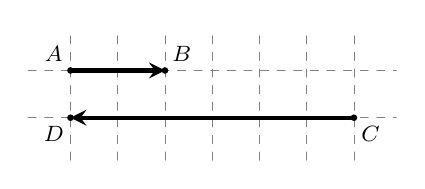
\begin{tikzpicture}[scale=1, font=\footnotesize, line join=round, line cap=round,>=stealth,xscale=0.6,yscale=0.6]
	\path (0,1)coordinate (A) (2,1) coordinate (B) (0,0) coordinate (D) (6,0) coordinate (C);
	\draw[step=1cm,gray,very thin,dashed] (-0.9,-0.9) grid (6.9,1.9);
	\draw[->,line width=1.5pt] (A)--(B);
	\draw[->,line width=1.5pt] (C)--(D);
	\foreach \p/\g in {A/135,B/45,C/-45,D/-135} \fill[black] (\p) circle(2pt)+(\g:0.5) node{$\p$};
	\end{tikzpicture}}
\loigiai{
	Hai vectơ $\overrightarrow{AB}$, $\overrightarrow{CD}$ ngược hướng và $CD=3AB$ nên $\overrightarrow{CD}=-3\overrightarrow{AB}$.
	}
\end{ex}
\begin{ex}%[0H5H3-2]%[Biên soạn tài liệu dạy học bộ KNTT-CS]%[Lê Minh Cường]
	\immini{
	Cho tam giác $ABC$ có đường trung tuyến $AM$, khẳng định nào sau đây đúng?
	\choice
	{$\overrightarrow{AM}=\overrightarrow{AB}+2\overrightarrow{BM}$}
	{\True $\overrightarrow{AM}=\dfrac{1}
	{2} \left(\overrightarrow{AB}+\overrightarrow{AC}\right)$}
	{$\overrightarrow{AM}=-\dfrac{1}{2} \left(\overrightarrow{AB}+\overrightarrow{AC}\right)$}
	{$\overrightarrow{AM}=\dfrac{1}{2} \left(\overrightarrow{AB}-\overrightarrow{AC}\right)$}
	}{
	\begin{tikzpicture}[line join=round, line cap=round,scale= 1,font=\footnotesize]
		\coordinate (A) at (-1,2);
		\coordinate (B) at (-2,0);
		\coordinate (C) at (3,0);
		\coordinate (M) at ($(B)!1/2!(C)$);
		\draw(A)--(B)--(C)--cycle;
		\draw(A)--(M) ;
		\foreach \i/\g in {A/90,B/-90,C/-90,M/-90}{\draw[fill=black](\i) circle (1pt) ($(\i)+(\g:3mm)$) node{$\i$};}
	\end{tikzpicture}
	}
\loigiai{
	Theo tính chất trung điểm đoạn thẳng ta có $\overrightarrow{AB}+\overrightarrow{AC}=2\overrightarrow{AM}$.\\
	Suy ra $\overrightarrow{AM}=\dfrac{1}{2} \left(\overrightarrow{AB}+\overrightarrow{AC}\right)$.
	}
\end{ex}
\begin{ex}%[0H5H3-2]%[Biên soạn tài liệu dạy học bộ KNTT-CS]%[Lê Minh Cường]
	\immini{
	Cho hình bình hành $ABCD$ tâm $O$. Khẳng định nào sau đây đúng?
	\choice
	{$\overrightarrow{AB}+\overrightarrow{AD}=3\overrightarrow{AO}$}
	{\True $2\overrightarrow{AB}+3\overrightarrow{AC}+2\overrightarrow{AD}=5\overrightarrow{AC}$}
	{$\overrightarrow{AB}+\overrightarrow{AD}=2\overrightarrow{AC}$}
	{$\overrightarrow{AB}+\overrightarrow{AC}+\overrightarrow{AD}=2\overrightarrow{AO}$}
	}{
	\begin{tikzpicture}[scale=1, font=\footnotesize, line join=round, line cap=round, >=stealth]
		\path	(0,0) coordinate (A)++(0:3) coordinate (B)
		($(B)+(60:2)$) coordinate (C)
		($(A)+(C)-(B)$) coordinate (D)
		($(A)!1/2!(C)$)coordinate (O)
		;
		\draw (A)--(B)--(C)--(D)--(A)--(C) (B)--(D);
		\foreach \x/\g in {A/-150,B/-30,C/30,O/-90,D/100}  \fill (\x) circle (1pt)+(\g:.3)node {$\x$};
	\end{tikzpicture}
	}
\loigiai{
	Theo quy tắc hình bình hành $\overrightarrow{AB}+\overrightarrow{AD}=\overrightarrow{AC}$ nên
	\[2\overrightarrow{AB}+3\overrightarrow{AC}+2\overrightarrow{AD}=2\left(\overrightarrow{AB}+\overrightarrow{AD}\right)+3\overrightarrow{AC}=2\overrightarrow{AC}+3\overrightarrow{AC}=5\overrightarrow{AC}.
	\]
	}
\end{ex}
\begin{ex}%[0H5N3-3]%[Biên soạn tài liệu dạy học bộ KNTT-CS]%[Lê Minh Cường]
	Trên đường thẳng $MN$ lấy điểm $P$ sao cho $\overrightarrow{MN}=-3\overrightarrow{MP}$. Điểm $P$ được xác định đúng theo hình vẽ nào sau đây.
	\choice
	{
	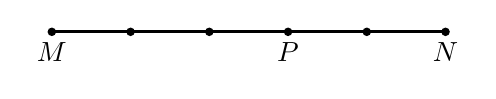
\begin{tikzpicture}[line width=1pt]
		\draw[-](0,0)--(5,0);
		\draw[fill=black](0,0) circle (1pt) node[below]{$M$};
		\draw[fill=black](1,0) circle (1pt);
		\draw[fill=black](2,0) circle (1pt);
		\draw[fill=black](3,0) circle (1pt) node[below]{$P$};
		\draw[fill=black](4,0) circle (1pt);
		\draw[fill=black](5,0) circle (1pt) node[below]{$N$};
	\end{tikzpicture}}
	{
	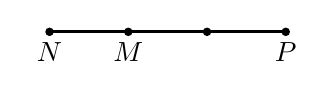
\begin{tikzpicture}[line width=1pt]
		\draw[-](8,0)--(11,0);
		\draw[fill=black](8,0) circle (1pt) node[below]{$N$};
		\draw[fill=black](9,0) circle (1pt) node[below]{$M$};
		\draw[fill=black](10,0) circle (1pt);
		\draw[fill=black](11,0) circle (1pt) node[below]{$P$};
	\end{tikzpicture}}
	{\True
	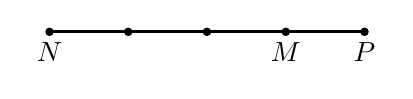
\begin{tikzpicture}[line width=1pt]
		\draw[-](0,0)--(4,0);
		\draw[fill=black](0,0) circle (1pt) node[below]{$N$};
		\draw[fill=black](1,0) circle (1pt);
		\draw[fill=black](2,0) circle (1pt);
		\draw[fill=black](3,0) circle (1pt) node[below]{$M$};
		\draw[fill=black](4,0) circle (1pt) node[below]{$P$};
	\end{tikzpicture}}
	{
	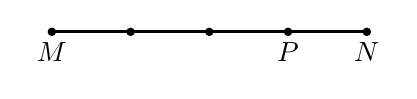
\begin{tikzpicture}[line width=1pt]
		\draw[-](8,0)--(12,0);
		\draw[fill=black](8,0) circle (1pt) node[below]{$M$};
		\draw[fill=black](9,0) circle (1pt);
		\draw[fill=black](10,0) circle (1pt);
		\draw[fill=black](11,0) circle (1pt) node[below]{$P$};
		\draw[fill=black](12,0) circle (1pt) node[below]{$N$};
	\end{tikzpicture}}
\loigiai{
	Vì $\overrightarrow{MN}=-3\overrightarrow{MP}$ nên $\overrightarrow{MN}$, $\overrightarrow{MP}$ ngược hướng và $MN=3MP$.
	}
\end{ex}
\begin{ex}%[0H5N3-3]%[Biên soạn tài liệu dạy học bộ KNTT-CS]%[Lê Minh Cường]
	Cho hình chữ nhật $ABCD$ có $AB=3, AD=4$. Giá trị của $\left|\overrightarrow{AC}\right|$ bằng
	\choice
	{$6$}
	{$3$}
	{$4$}
	{\True $5$}
\loigiai{
	\immini
	{
	Ta có $\left|\overrightarrow{AC}\right|=AC=\sqrt{AB^2+BC^2}=\sqrt{AB^2+AD^2}=5$.
	}
	{
	\begin{tikzpicture}[line join = round, line cap = round,>=stealth,font=\footnotesize,scale=.6]
		\tkzDefPoints{0/0/D}
		\coordinate (C) at ($(D)+(3,0)$);
		\coordinate (A) at ($(D)+(0,4)$);
		\coordinate (B) at ($(A)+(C)-(D)$);
		\draw (A)--(B)--(C)--(D)--(A);
		\draw[->] (A)--(C);
		\foreach \p/\q in {A/90,B/90,C/-90,D/-90}
		\fill[black] (\p)node[shift={(\q:3mm)}]{$\p$} circle (1.0pt);
	\end{tikzpicture}
	}
	}
\end{ex}
\begin{ex}%[0H5N3-3]%[Biên soạn tài liệu dạy học bộ KNTT-CS]%[Lê Minh Cường]
	Cho tam giác đều $ABC$ với đường cao $AH$. Mệnh đề nào sau đây đúng?
	\choice
	{$\overrightarrow{AB}=\overrightarrow{AC}$}
	{$\left|\overrightarrow{AH}\right|=\dfrac{\sqrt{3}}
	{2}\left|\overrightarrow{HC}\right|$}
	{$\overrightarrow{HB}=\overrightarrow{HC}$}
	{\True $\left|\overrightarrow{AC}\right|=2\left|\overrightarrow{HC}\right|$}
\loigiai{
	\immini
	{
	Ta có $2\left|\overrightarrow{HC}\right|=\left|\overrightarrow{BC}\right|=BC=AC=\left|\overrightarrow{AC}\right|$.
	}
	{
	\begin{tikzpicture}[line join = round, line cap = round, scale=1]
		\def \a{2.5};
		\coordinate (B) at (0,0);
		\coordinate (C) at ($(B)+(\a,0)$);
		\coordinate[ shift=(60:\a cm)] (A) at (B);
		\coordinate (H) at ($(B)!0.5!(C)$);
		\draw (A)--(B)--(C)--cycle (A)--(H);
		\foreach \x in {A,B,C,H} \fill[black] (\x) circle (1.2pt);
		\draw pic[draw, angle radius=0.2cm]{right angle=A--H--B};
		\foreach \p/\q in {A/90,B/180,C/0,H/-90}
		\fill[black] (\p)node[shift={(\q:3mm)}]{$\p$} circle (1.0pt);
	\end{tikzpicture}
	}
	}
\end{ex}
\begin{ex}%[0H5N3-3]%[Biên soạn tài liệu dạy học bộ KNTT-CS]%[Lê Minh Cường]
	Cho hình thoi $ABCD$ tâm $O,$ cạnh bằng $a$ và góc $A$ bằng $60^{\circ}.$ Kết luận nào đúng?
	\choice
	{$|\overrightarrow{OA}|=|\overrightarrow{OB}|$}
	{$|\overrightarrow{OA}|=a$}
	{\True $|\overrightarrow{OA}|=\dfrac{a \sqrt{3}}
	{2}$}
	{$|\overrightarrow{OA}|=\dfrac{a \sqrt{2}}{2}$}
\loigiai{
	\immini
	{
	Ta có $\triangle ABD$ là tam giác đều cạnh $a$ nên $|\overrightarrow{OA}|=OA=\dfrac{a \sqrt{3}}{2}$.
	}
	{
	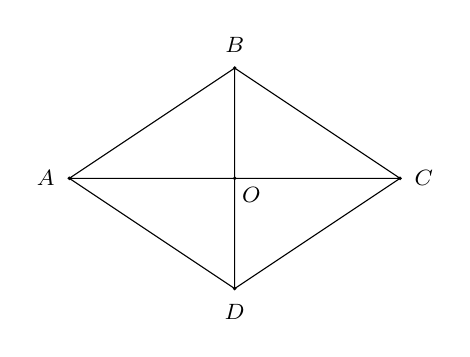
\begin{tikzpicture}[line join = round, line cap = round,>=stealth,font=\footnotesize,scale=0.7]
		\def\gocA{60} \def\a{3} \def\b{2} %độ dài cạnh
		\path
		(-180:\a) coordinate(A)
		(0:\a)coordinate(C)
		(90:\b) coordinate (B)
		(-90:\b)coordinate (D)
		(0:0)coordinate (O)
		;
		%
		\draw (A)--(B)--(C)--(D)--(A) (A)--(C) (B)--(D);
		\foreach \p/\q in {A/180,B/90,C/0,D/-90,O/-45}
		\fill[black] (\p)node[shift={(\q:3mm)}]{$\p$} circle (1.0pt);
	\end{tikzpicture}
	}
	}
\end{ex}
\begin{ex}%[0H5N3-3]%[Biên soạn tài liệu dạy học bộ KNTT-CS]%[Lê Minh Cường]
	Cho hình chữ nhật $ABCD$, gọi $O$ là giao điểm của $AC$ và $BD$. Mệnh đề nào sau đây đúng?
	\choice
	{$\overrightarrow{OA}=\overrightarrow{OB}=\overrightarrow{OC}=\overrightarrow{OD}$}
	{$\overrightarrow{AC}=\overrightarrow{BD}$}
	{$\left|\overrightarrow{OA}+\overrightarrow{OB}+\overrightarrow{OC}+\overrightarrow{OD}\right|=\overrightarrow{0}$}
	{\True $\overrightarrow{AC}-\overrightarrow{AD}=\overrightarrow{AB}$}
\loigiai{
	\immini
	{
	Ta có $\overrightarrow{AC}-\overrightarrow{AD}=\overrightarrow{DC}=\overrightarrow{AB}$.
	}
	{
	\begin{tikzpicture}[line join = round, line cap = round,>=stealth,font=\footnotesize,scale=.6]
		\coordinate (D) at (0,0);
		\coordinate (C) at ($(D)+(5,0)$);
		\coordinate (A) at ($(D)+(0,3)$);
		\coordinate (B) at ($(A)+(C)-(D)$);
		\coordinate (O) at ($(A)!0.5!(C)$);
		\draw (A)--(C) (B)--(D)
		(A)--(B)--(C)--(D)--(A);
		\foreach \p/\q in {A/90,B/90,C/-90,D/-90,O/-90}
		\fill[black] (\p)node[shift={(\q:3mm)}]{$\p$} circle (1.0pt);
	\end{tikzpicture}
	}
	}
\end{ex}
\begin{ex}%[0H5N3-3]%[Biên soạn tài liệu dạy học bộ KNTT-CS]%[Lê Minh Cường]
	Cho tam giác $ABC$ vuông tại $A$ có $AB=3, BC=5$. Tính $\left|\overrightarrow{AB}+\overrightarrow{BC}\right|$.
	\choice
	{\True $4$}
	{$5$}
	{$6$}
	{$3$}
\loigiai{
	\immini
	{
	Ta có $\left|\overrightarrow{AB}+\overrightarrow{BC}\right|=\left|\overrightarrow{AC}\right|=AC=\sqrt{BC^2-AB^2}=4$.
	}
	{
	\begin{tikzpicture}[line join = round, line cap = round, scale=.6]
		\coordinate[label = left:$A$] (A) at (0,0);
		\coordinate[label = right:$B$] (B) at ($(A)+(3,0)$);
		\coordinate[label = above:$C$] (C) at ($(A)+(0,4)$);
		\draw pic[draw, angle radius=0.2cm]{right angle=C--A--B};
		\draw (A)--(B)--(C)--cycle;
		\foreach \x in {A,B,C} \fill[black] (\x) circle (1.5pt);
	\end{tikzpicture}
	}
	}
\end{ex}
\begin{ex}%[0H5H3-5]%[Biên soạn tài liệu dạy học bộ KNTT-CS]%[Lê Minh Cường]
	Cho tam giác $ABC$. Gọi $M$ là điểm trên cạnh $BC$ sao cho $MB = 4MC$. Khi đó
	\choice
	{$\overrightarrow{AM} = \dfrac{4}
	{5} \overrightarrow{AB} + \dfrac{1}
	{5} \overrightarrow{AC}$}
	{$\overrightarrow{AM} = \dfrac{4}{5} \overrightarrow{AB} - \overrightarrow{AC}$}
	{$\overrightarrow{AM} = \dfrac{4}{5} \overrightarrow{AB} - \dfrac{1}{5} \overrightarrow{AC}$}
	{\True $\overrightarrow{AM} = \dfrac{1}{5} \overrightarrow{AB} + \dfrac{4}{5} \overrightarrow{AC}$}
\loigiai{
	\immini{
	\begin{align*}
		\overrightarrow{AM} &= \overrightarrow{AB} + \overrightarrow{BM} = \overrightarrow{AB} + \dfrac{4}{5} \overrightarrow{BC} \\
		&= \overrightarrow{AB} + \dfrac{4}{5} \left(\overrightarrow{BA} + \overrightarrow{AC}\right) \\
		&= \dfrac{1}{5} \overrightarrow{AB} + \dfrac{4}{5} \overrightarrow{AC}.
	\end{align*}
	}{
	\begin{tikzpicture}[>=stealth,line join=round,line cap=round,font=\footnotesize,scale=1]
		\tikzset{
		pics/tamgiacbg/.style n args={3}{
		code={
		\tikzset{
		% Khai báo độ dài cạnh va 2 goc
		declare function={a=4;goc1=70;goc2=-40;}
		}
		% Vẽ tam giác
		\path (0,0)coordinate (#1)--+(0:a)coordinate (#2)
		($(#1)!{sin(goc1)*.2}!{goc1}:(#2)$)coordinate (x)
		($(#2)!{sin(goc2)*.2}!{goc2}:(#1)$)coordinate (y)
		(intersection of #1--x and #2--y)coordinate (#3)
		;
		\foreach \pointo/\pointt in {#1/#3,#1/#2,#2/#3}{
		\draw[fill=black](\pointo)--(\pointt);
		}
		}
		}
		}
		\path
		(0,0)pic{tamgiacbg={B}{C}{A}}
		($(B)!4/5!(C)$)coordinate (M)
		;
		\foreach \pointo/\pointt in {A/M}{
		\draw[fill=black](\pointo)--(\pointt);
		}
		\foreach \point/\goc in {A/90,B/190,C/-10,M/-90}{
		\draw[fill=black](\point)circle(.8pt)+(\goc:2mm)node[scale=.8]{$\point$};
		}
	\end{tikzpicture}
	}
	}
\end{ex}
\begin{ex}%[0H5H3-5]%[Biên soạn tài liệu dạy học bộ KNTT-CS]%[Lê Minh Cường]
	Cho tam giác $ABC$. Điểm $I$ trên cạnh $AC$ sao cho $CI = \dfrac{1}{4} CA$. Phân tích $\overrightarrow{BI}$ theo hai vectơ $\overrightarrow{AB}$ và $\overrightarrow{AC}$. Khẳng định nào sau đây đúng?
	\choice
	{\True $\overrightarrow{BI} = \dfrac{1}
	{4} \overrightarrow{AC} - \overrightarrow{AB}$}
	{$\overrightarrow{BI} = \dfrac{3}
	{4} \overrightarrow{AC} - \overrightarrow{AB}$}
	{$\overrightarrow{BI} = \dfrac{5}{4} \overrightarrow{AC} + \overrightarrow{AB}$}
	{$\overrightarrow{BI} = \dfrac{3}{4} \overrightarrow{AC} + \overrightarrow{AB}$}
\loigiai{
	\immini{
	Ta có $CI=\dfrac{1}{4}CA$ nên $AI=\dfrac{3}{4}AC$.\\
	Khi đó \[\overrightarrow{BI}=\overrightarrow{BA}+\overrightarrow{AI}=-\overrightarrow{AB}+\dfrac{1}{4}\overrightarrow{AC}.\]
	}{
	\begin{tikzpicture}[>=stealth,line join=round,line cap=round,font=\footnotesize,scale=1]
		\tikzset{
		pics/tamgiacbg/.style n args={3}{
		code={
		\tikzset{
		% Khai báo độ dài cạnh va 2 goc
		declare function={a=4;goc1=70;goc2=-40;}
		}
		% Vẽ tam giác
		\path (0,0)coordinate (#1)--+(0:a)coordinate (#2)
		($(#1)!{sin(goc1)*.2}!{goc1}:(#2)$)coordinate (x)
		($(#2)!{sin(goc2)*.2}!{goc2}:(#1)$)coordinate (y)
		(intersection of #1--x and #2--y)coordinate (#3)
		;
		\foreach \pointo/\pointt in {#1/#3,#1/#2,#2/#3}{
		\draw[fill=black](\pointo)--(\pointt);
		}
		}
		}
		}
		\path
		(0,0)pic{tamgiacbg={B}{C}{A}}
		($(C)!1/4!(A)$)coordinate (I)
		;
		\foreach \pointo/\pointt in {B/I}{
		\draw[fill=black](\pointo)--(\pointt);
		}
		\foreach \point/\goc in {A/90,B/190,C/-10,I/45}{
		\draw[fill=black](\point)circle(.8pt)+(\goc:2mm)node[scale=.8]{$\point$};
		}
	\end{tikzpicture}
	}
	}
\end{ex}
\begin{ex}%[0H5H3-5]%[Biên soạn tài liệu dạy học bộ KNTT-CS]%[Lê Minh Cường]
	Cho tứ giác $ABCD$. Trên cạnh $AB, CD$ lấy lần lượt các điểm $M, N$ sao cho $3\overrightarrow{AM} = 2\overrightarrow{AB}$ và $3\overrightarrow{DN} = 2\overrightarrow{DC}$. Tính vectơ $\overrightarrow{MN}$ theo hai vectơ $\overrightarrow{AD}$ và $\overrightarrow{BC}$.
	\choice
	{$\overrightarrow{MN} = \dfrac{1}
	{3}\overrightarrow{AD} + \dfrac{1}
	{3}\overrightarrow{BC}$}
	{$\overrightarrow{MN} = \dfrac{1}{3}\overrightarrow{AD} - \dfrac{2}{3}\overrightarrow{BC}$}
	{\True $\overrightarrow{MN} = \dfrac{1}{3}\overrightarrow{AD} + \dfrac{2}{3}\overrightarrow{BC}$}
	{$\overrightarrow{MN} = \dfrac{2}{3}\overrightarrow{AD} + \dfrac{1}{3}\overrightarrow{BC}$}
\loigiai{
	\immini{
	Ta có $\overrightarrow{MN} = \overrightarrow{MA} + \overrightarrow{AD} + \overrightarrow{DN}$ và $\overrightarrow{MN} = \overrightarrow{MB} + \overrightarrow{BC} + \overrightarrow{CN}$. \\
	Suy ra
	\allowdisplaybreaks
	\begin{eqnarray*}
		3\overrightarrow{MN} &=& \overrightarrow{MA} + \overrightarrow{AD} + \overrightarrow{DN} + 2(\overrightarrow{MB} + \overrightarrow{BC} + \overrightarrow{CN})\\
		&=& (\overrightarrow{MA} + 2\overrightarrow{MB}) + \overrightarrow{AD} + 2\overrightarrow{BC} + (\overrightarrow{DN} + 2\overrightarrow{CN}).
	\end{eqnarray*}
	Theo bài ra, ta có $\overrightarrow{MA} + 2\overrightarrow{MB} = \overrightarrow{0}$ và $\overrightarrow{DN} + 2\overrightarrow{CN} = \overrightarrow{0}$.\\
	Vậy $3\overrightarrow{MN} = \overrightarrow{AD} + 2\overrightarrow{BC} \Rightarrow \overrightarrow{MN} = \dfrac{1}{3}\overrightarrow{AD} + \dfrac{2}{3}\overrightarrow{BC}$.
	}{\begin{tikzpicture}[>=stealth,line join=round,line cap=round,font=\footnotesize,scale=1]
	\draw (0,0)coordinate (A)--++(-10:3)coordinate (B)--++(-120:2)coordinate (C)--++(180:2.5)coordinate (D)--cycle
	($(A)!2/3!(B)$)coordinate (M)--($(D)!2/3!(C)$)coordinate (N)
	;
	\foreach \point/\goc in {A/120,B/30,C/-20,D/190,M/90,N/-90}{
	\draw[fill=black](\point)circle(.8pt)+(\goc:2mm)node[scale=.8]{$\point$};
	}
	\end{tikzpicture}
	}
	}
\end{ex}
\Closesolutionfile{ans}
\indapan{6}{ans/ans-c4b9-lc}
%---------------------Trắc nghiệm đúng sai
\ind{PHẦN II.} \inden{Câu trắc nghiệm đúng sai. Trong mỗi ý a), b), c), d) ở mỗi câu, học sinh chọn đúng hoặc sai.}
\setcounter{ex}{0}
\Opensolutionfile{ans}[ans/ans-c4b9-ds]
\begin{ex}%[0H5H3-2]%[Biên soạn tài liệu dạy học bộ KNTT-CS]%[Lê Minh Cường]
	Cho tam giác $ABC$ có trọng tâm $G$ và $M$ là trung điểm của $BC$. Các mệnh đề sau đúng hay sai?
	\choiceTF
	{\True $\overrightarrow{GA}=2\overrightarrow{MG}$}
	{\True $\overrightarrow{AG}=\dfrac{2}{3}\overrightarrow{AM}$}
	{$\overrightarrow{AG}=2\overrightarrow{MG}$}
	{$\overrightarrow{AM}=3\overrightarrow{MG}$}
\loigiai{
	\immini{\begin{itemchoice}
	\itemch Ta có $GA=2GM$ và $\overrightarrow{GA}$, $\overrightarrow{MG}$ cùng hướng nên $\overrightarrow{GA}=2\overrightarrow{MG}$.
	\itemch Ta có $GA=\dfrac{2}{3}AM$ và $\overrightarrow{AG}$ và $\overrightarrow{AM}$ cùng hướng nên $\overrightarrow{AG}=\dfrac{2}{3}\overrightarrow{AM}$.
	\itemch Ta có $AG=2MG$ và $\overrightarrow{GA}$, $\overrightarrow{MG}$ ngược hướng nên $\overrightarrow{AG}=2\overrightarrow{MG}$ là sai.
	\itemch Ta có $MA=3GM$ và $\overrightarrow{AM}$, $\overrightarrow{MG}$ ngược hướng nên $\overrightarrow{AM}=3\overrightarrow{MG}$ là sai.
	\end{itemchoice}}{			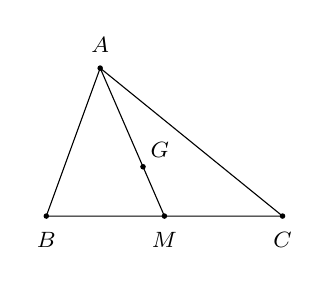
\begin{tikzpicture}[scale=1,>=stealth, font=\footnotesize, line join=round, line cap=round,declare function={h=2;}]
	\path
	(0,0) coordinate (B)
	(3,0) coordinate (C)
	(B)+(70:h) coordinate (A)
	(barycentric cs:C=1,B=1)coordinate(M)
	(barycentric cs:A=1,B=1,C=1)coordinate(G)
	;
	\draw (A)--(B)--(C)--(A)--(M);
	\foreach \p/\g in {A/90,B/-90,C/-90,M/-90,G/45} \fill[black] (\p) circle(1pt)+(\g:0.3) node{$\p$};
	\end{tikzpicture}}
	}
\end{ex}
\begin{ex}%[0H5H3-3]%[Biên soạn tài liệu dạy học bộ KNTT-CS]%[Lê Minh Cường]
	Cho tam giác $ABC$, $N$ là trung điểm $AB$, $M$ là điểm thỏa mãn đẳng thức $\overrightarrow{MN}= \dfrac{1}{2} \overrightarrow{AB} + \overrightarrow{AC}$. Xét tính đúng sai của các mệnh đề sau.
	\choiceTF
	{\True $\overrightarrow{NA}+\overrightarrow{NB}=\overrightarrow{0}$}
	{$\dfrac{1}{2} \overrightarrow{AB} = \overrightarrow{NA}$}
	{\True $\overrightarrow{AM}+\overrightarrow{AC} = \overrightarrow{0}$}
	{\True $M$ đối xứng với $C$ qua $A$}
\loigiai{
	\immini
	{
	Ta có
	\begin{eqnarray*}
		& &	\overrightarrow{MN}= \dfrac{1}{2} \overrightarrow{AB} + \overrightarrow{AC} \Leftrightarrow \overrightarrow{MN}= \overrightarrow{AN} + \overrightarrow{AC} \\
		& \Leftrightarrow & \overrightarrow{MN}+\overrightarrow{NA} = \overrightarrow{AC}  \Leftrightarrow  \overrightarrow{AM}+\overrightarrow{AC} = \overrightarrow{0}.
	\end{eqnarray*}
	Suy ra $A$ là trung điểm $MC$ hay $M$ đối xứng với $C$ qua $A$.
	}
	{
	\begin{tikzpicture}[scale=0.6,>=stealth, font=\footnotesize, line join=round, line cap=round]
		\foreach \ten/\x/\y in {B/0/0,C/3/0,A/2,2}{
		\coordinate (\ten) at (\x,\y); }
		\coordinate (N) at ($(A)!0.5!(B)$);
		\coordinate (M) at ($(A)!-1!(C)$);
		\draw (A)--(B)--(C)--(M);
		\foreach \p/\r in {A/90,C/0,B/180,N/150,M/30}
		\fill (\p) circle (1pt) node[shift={(\r:3mm)}]{$\p$};
	\end{tikzpicture}
	}
	\begin{itemchoice}
		\itemch  Ta có  $N$ là trung điểm $AB$ nên $\overrightarrow{NA}+\overrightarrow{NB}=\overrightarrow{0}$.
		\itemch Ta có  $N$ là trung điểm $AB$ nên $\dfrac{1}{2} \overrightarrow{AB} = \overrightarrow{AN}$.
		\itemch Ta có $A$ là trung điểm của $MC$ nên $\overrightarrow{AM}+\overrightarrow{AC} = \overrightarrow{0}$
		\itemch Ta có $A$ là trung điểm của $MC$ nên  $M$ đối xứng với $C$ qua $A$.
	\end{itemchoice}
	}
\end{ex}
\begin{ex}%[0H5H3-9]%[Biên soạn tài liệu dạy học bộ KNTT-CS]%[Lê Minh Cường]
	Máy bay $A$ đang bay về hướng đông bắc với tốc độ $600$ km/h. Cùng lúc đó, máy bay $B$ đang bay về hướng tây nam với tốc độ $800$ km/h (như hình vẽ).
	\begin{center}
		\begin{tikzpicture}[scale=1,>=stealth, font=\footnotesize, line join=round, line cap=round,declare function={a=2;h=1;db=15;tn=-135;}]
			%------------máy bay
			\tikzset{maybay/.pic={
			%Đuôi máy bay
			\def\D{  (-2,-.45)--(-2.36,.24)--(-2.2,.3)--(-1.35,-.25)--cycle
			;}
			\draw \D;
			\fill[brown!40!] \D;
			%Quạt máy bay
			\def\Q{  (.15,-.1)
			..controls +(-140:0.1) and +(140:0.1) .. (.2,-.35)--(.8,-.17)--(.7,.07)--cycle
			;}
			\draw \Q;
			\draw[xshift=.5cm] \Q;
			\fill[brown!40!,xshift=.5cm] \Q;
			%---------elip2
			\draw[rotate=-70,xshift=-.23cm,yshift=1.27cm] (.7,-.1) ellipse (.12cm and .07cm);
			%Thân máy bay
			\def\T{  (-2.1,-.5)
			..controls +(40:0) and +(-170:0.7) .. (2,.74)
			..controls +(-40:0) and +(170:0.3) .. (2.55,.7)
			..controls +(-150:0) and +(30:.65) .. (2.1,.3)
			..controls +(-150:0) and +(-18:1.25) .. (-2.1,-.6)
			..controls +(90:0) and +(-90:0) .. (-2.1,-.51)
			-- (-2.5,-.52)--cycle;
			}
			\draw \T;
			\fill[brown!70!] \T;
			%Cánh máy bay
			\def\C{  (.5,.05)
			..controls +(170:0) and +(-10:0) .. (-1.48,.12)
			..controls +(-80:0) and +(170:0.02) .. (-1.65,.3)
			..controls +(180:0) and +(0:0) .. (-1.77,.3)
			..controls +(-80:0) and +(110:0) .. (-1.64,.12)
			..controls +(-35:0) and +(145:0) .. (-.2,-.17)
			--cycle
			;}
			\draw \C;
			\fill[brown!40!] \C;
			%Quạt sau
			\fill[brown!40!] \Q;
			%----elip 1
			\draw[rotate=-70,xshift=-.4cm,yshift=.8cm] (.7,-.1) ellipse (.12cm and .07cm);
			%Ô cửa
			\draw (2.18,0.73)--(2.5,0.7)--(2.14,0.58)--cycle;
			\fill[brown!40!](2.18,0.73)--(2.51,0.71)--(2.14,0.57)--cycle;
			}}
			\path
			(2,1) coordinate (A)
			(A)+(0.5,0.4)coordinate (M)
			(M)+(db+17:0.9)coordinate (N)
			(A)+(2,-h) coordinate (B)
			(B)+(-0.4,-0.1)coordinate (P)
			(P)+(tn-17:1.2)coordinate (Q)
			(A)+(-2,-1)coordinate (O)
			(O)+(-0.8,0)coordinate (x')
			(O)+(0.8,0)coordinate (x)
			(O)+(0,-0.8)coordinate (y')
			(O)+(0,0.8)coordinate (y)
			;
			\path(A) pic[shift={(80:.15)},scale=.2,rotate=db,yscale=1]{maybay};
			\path(B) pic[shift={(80:.15)},scale=.2,rotate=tn,yscale=-1]{maybay};
			\draw[-stealth](M)--(N);
			\draw[-stealth](P)--(Q);
			\path ($(M)!0.5!(N)$)node[shift={(90:.25)},scale=1]{$\overrightarrow{a}$};
			\path ($(P)!0.5!(Q)$)node[shift={(-90:.25)},scale=1]{$\overrightarrow{b}$};
			\foreach \p/\g in{A/-60,B/-60}
			\path(\p)node[shift={(\g:.2)},scale=1]{$\p$};
			%%%%La bàn
			\draw[-stealth,line width=1.5pt](O)--(x')node[shift={(-180:.4)},scale=1]{Tây};
			\draw[-stealth,line width=1.5pt](O)--(x)node[shift={(0:.5)},scale=1]{Đông};
			\draw[-stealth,line width=1.5pt](O)--(y')node[shift={(-90:.2)},scale=1]{Nam};
			\draw[-stealth,line width=1.5pt](O)--(y)node[shift={(90:.2)},scale=1]{Bắc};
			\draw[fill=white,line width=1.5pt](O)circle(0.15);
			\shade[shading=ball](O)circle(.05);
		\end{tikzpicture}
	\end{center}
	Các mệnh đề sau đúng hay sai?
	\choiceTF
	{\True vectơ vận tốc $\overrightarrow{b}$ của máy bay $B$ ngược hướng với vectơ vận tốc $\overrightarrow{a}$ của máy bay $A$}
	{$\left|\overrightarrow{a}\right|=800$ km/h, $\left|\overrightarrow{b}\right|=600$ km/h}
	{\True $\overrightarrow{b}=\dfrac{-4}{3}\overrightarrow{a}$}
	{$\overrightarrow{a}=\dfrac{4}{3}\overrightarrow{b}$}
\loigiai{
	Ta thấy hướng đông bắc ngược hướng với hướng tây nam.
	\begin{itemchoice}
		\itemch vectơ vận tốc $\overrightarrow{b}$ của máy bay $B$ ngược hướng với vectơ vận tốc $\overrightarrow{a}$ của máy bay $A$.\hfill $(1)$
		\itemch Theo đề bài ta có $\left|\overrightarrow{a}\right|=600$ km/h, $\left|\overrightarrow{b}\right|=800$ km/h nên $\dfrac{\left|\overrightarrow{b}\right|}{\left|\overrightarrow{a}\right|}=\dfrac{800}{600}=\dfrac{4}{3}$.\\
		Suy ra $\left|\overrightarrow{b}\right|=\dfrac{4}{3}\left|\overrightarrow{a}\right|$.\hfill $(2)$
		\itemch Từ $(1)$ và $(2)$ suy ra $\overrightarrow{b}=\dfrac{-4}{3}\overrightarrow{a}$.
		\itemch Từ $(1)$ và $(2)$ suy ra $\overrightarrow{b}=\dfrac{-4}{3}\overrightarrow{a}$.
	\end{itemchoice}
	}
\end{ex}
\begin{ex}%[0H5H3-9]%[Biên soạn tài liệu dạy học bộ KNTT-CS]%[Lê Minh Cường]
	Máy bay $A$ đang bay về hướng đông bắc với tốc độ $300$ km/h. Cùng lúc đó, máy bay $B$ đang bay về hướng tây nam với tốc độ $350$ km/h (như hình vẽ).
	\begin{center}
		\begin{tikzpicture}[scale=1,>=stealth, font=\footnotesize, line join=round, line cap=round,declare function={a=2;h=1;db=15;tn=-135;}]
			%------------máy bay
			\tikzset{maybay/.pic={
			%Đuôi máy bay
			\def\D{  (-2,-.45)--(-2.36,.24)--(-2.2,.3)--(-1.35,-.25)--cycle
			;}
			\draw \D;
			\fill[cyan!40!] \D;
			%Quạt máy bay
			\def\Q{  (.15,-.1)
			..controls +(-140:0.1) and +(140:0.1) .. (.2,-.35)--(.8,-.17)--(.7,.07)--cycle
			;}
			\draw \Q;
			\draw[xshift=.5cm] \Q;
			\fill[cyan!40!,xshift=.5cm] \Q;
			%---------elip2
			\draw[rotate=-70,xshift=-.23cm,yshift=1.27cm] (.7,-.1) ellipse (.12cm and .07cm);
			%Thân máy bay
			\def\T{  (-2.1,-.5)
			..controls +(40:0) and +(-170:0.7) .. (2,.74)
			..controls +(-40:0) and +(170:0.3) .. (2.55,.7)
			..controls +(-150:0) and +(30:.65) .. (2.1,.3)
			..controls +(-150:0) and +(-18:1.25) .. (-2.1,-.6)
			..controls +(90:0) and +(-90:0) .. (-2.1,-.51)
			-- (-2.5,-.52)--cycle;
			}
			\draw \T;
			\fill[blue!70!] \T;
			%Cánh máy bay
			\def\C{  (.5,.05)
			..controls +(170:0) and +(-10:0) .. (-1.48,.12)
			..controls +(-80:0) and +(170:0.02) .. (-1.65,.3)
			..controls +(180:0) and +(0:0) .. (-1.77,.3)
			..controls +(-80:0) and +(110:0) .. (-1.64,.12)
			..controls +(-35:0) and +(145:0) .. (-.2,-.17)
			--cycle
			;}
			\draw \C;
			\fill[cyan!40!] \C;
			%Quạt sau
			\fill[cyan!40!] \Q;
			%----elip 1
			\draw[rotate=-70,xshift=-.4cm,yshift=.8cm] (.7,-.1) ellipse (.12cm and .07cm);
			%Ô cửa
			\draw (2.18,0.73)--(2.5,0.7)--(2.14,0.58)--cycle;
			\fill[cyan!40!](2.18,0.73)--(2.51,0.71)--(2.14,0.57)--cycle;
			}}
			\path
			(2,1) coordinate (A)
			(A)+(0.5,0.4)coordinate (M)
			(M)+(db+17:0.9)coordinate (N)
			(A)+(2,-h) coordinate (B)
			(B)+(-0.4,-0.1)coordinate (P)
			(P)+(tn-17:1.2)coordinate (Q)
			(A)+(-2,-1)coordinate (O)
			(O)+(-0.8,0)coordinate (x')
			(O)+(0.8,0)coordinate (x)
			(O)+(0,-0.8)coordinate (y')
			(O)+(0,0.8)coordinate (y)
			;
			\path(A) pic[shift={(80:.15)},scale=.2,rotate=db,yscale=1]{maybay};
			\path(B) pic[shift={(80:.15)},scale=.2,rotate=tn,yscale=-1]{maybay};
			\draw[-stealth](M)--(N);
			\draw[-stealth](P)--(Q);
			\path ($(M)!0.5!(N)$)node[shift={(90:.25)},scale=1]{$\overrightarrow{a}$};
			\path ($(P)!0.5!(Q)$)node[shift={(-90:.25)},scale=1]{$\overrightarrow{b}$};
			\foreach \p/\g in{A/-60,B/-60}
			\path(\p)node[shift={(\g:.2)},scale=1]{$\p$};
			%%%%La bàn
			\draw[-stealth,line width=1.5pt](O)--(x')node[shift={(-180:.4)},scale=1]{Tây};
			\draw[-stealth,line width=1.5pt](O)--(x)node[shift={(0:.5)},scale=1]{Đông};
			\draw[-stealth,line width=1.5pt](O)--(y')node[shift={(-90:.2)},scale=1]{Nam};
			\draw[-stealth,line width=1.5pt](O)--(y)node[shift={(90:.2)},scale=1]{Bắc};
			\draw[fill=white,line width=1.5pt](O)circle(0.15);
			\shade[shading=ball](O)circle(.05);
		\end{tikzpicture}
	\end{center}
	Xét tính đúng sai của các khẳng định sau:
	\choiceTF
	{\True vectơ vận tốc $\overrightarrow{b}$ của máy bay $B$ ngược hướng với vectơ vận tốc $\overrightarrow{a}$ của máy bay $A$}
	{\True $|\overrightarrow{a}|=\dfrac{6}{7}|\overrightarrow{b}|$}
	{$\overrightarrow{b}=\dfrac{7}{6}\overrightarrow{a}$}
	{$\big|\overrightarrow{a}+\overrightarrow{b}\big|=750$ (km/h)}
\loigiai{
	\begin{itemchoice}
		\itemch Khẳng định đúng. hai vectơ vận tốc của hai máy bay $A$ và $B$ ngược hướng nhau.
		\itemch Khẳng định đúng.\\
		Ta có $|\overrightarrow{a}|=300$; $|\overrightarrow{b}|=350$. Ta thấy $\dfrac{|\overrightarrow{a}|}{|\overrightarrow{b}|}=\dfrac{300}{350}=\dfrac{6}{7}\Rightarrow |\overrightarrow{a}|=\dfrac{6}{7}|\overrightarrow{b}|$.
		\itemch Khẳng định sai. Ta có $\heva{&|\overrightarrow{a}|=\dfrac{6}{7}|\overrightarrow{b}|\\
		&\overrightarrow{a}\,\text{và}\,\overrightarrow{b}\,\text{ngược hướng}}\Rightarrow \heva{&|\overrightarrow{b}|=\dfrac{7}{6}|\overrightarrow{a}|\\&\overrightarrow{a}\,\text{và}\,\overrightarrow{b}\,\text{ngược hướng}}\Rightarrow \overrightarrow{b}=-\dfrac{7}{6}\overrightarrow{a}$.
		\itemch Khẳng định sai.\\
		Ta có $\big|\overrightarrow{a}+\overrightarrow{b}\big|=350-300=50$ (km/h).
	\end{itemchoice}
	}
\end{ex}
\Closesolutionfile{ans}
\indapan{3}{ans/ans-c4b9-ds}
%---------------Trắc nghiệm trả lời ngắn
\ind{PHẦN III.} \inden{Câu trả lời ngắn.}
\setcounter{ex}{0}
\Opensolutionfile{ans}[ans/ans-c4b9-kq]
\begin{ex}%[0H5H3-2]%[Biên soạn tài liệu dạy học bộ KNTT-CS]%[Lê Minh Cường]
	Cho tam giác $JPH$ đều tâm $B$; $M$ là điểm bất kỳ trong tam giác. Hình chiếu của $M$ xuống ba cạnh lần lượt là $D$, $E$, $F$. Khi đó ta được hệ thức $\overrightarrow{MD}+\overrightarrow{ME}+\overrightarrow{MF}=\dfrac{a}{2} \overrightarrow{MB}$. Tìm $a$?
	\par\shortans{$3$}
\loigiai{
	\begin{center}
		\begin{tikzpicture}[scale=0.8,>=stealth,line join=round,line cap=round,font=\footnotesize]
			\def\a{6}
			\path (0:0) coordinate (P)
			++(0:{\a}) coordinate (H)
			([turn]120:{\a}) coordinate (J)
			++(-100:{\a/2}) coordinate (M)
			($(P)!(M)!(H)$) coordinate (D)
			($(J)!(M)!(H)$) coordinate (E)
			($(J)!(M)!(P)$) coordinate (F)
			($(M)+(H)-(P)$) coordinate (X)
			($(M)+(J)-(P)$) coordinate (Y)
			($(M)+(J)-(H)$) coordinate (Z)
			(intersection of Y--M and J--H) coordinate (A_1)
			(intersection of Y--M and P--H) coordinate (B_1)
			(intersection of Z--M and J--P) coordinate (A_2)
			(intersection of Z--M and P--H) coordinate (C_1)
			(intersection of X--M and J--P) coordinate (B_2)
			(intersection of X--M and J--H) coordinate (C_2);
			\draw (J)--(P)--(H)--cycle (B_1)--(A_1) (A_2)--(C_1) (B_2)--(C_2);
			\draw[dashed,thick] (M)--(D) (M)--(E) (M)--(F);
			\draw pic[draw,angle radius=2mm]{right angle=H--D--M};
			\draw pic[draw,angle radius=2mm]{right angle=M--F--J};
			\draw pic[draw,angle radius=2mm]{right angle=J--E--M};
			\foreach \x/ \goc in {J/135,P/-135,H/-45,D/-90,E/0,F/160,A_1/0,B_1/-90,C_1/-90,A_2/160,B_2/160,C_2/0}
			\fill (\x) circle (1.5pt) ($(\x)+(\goc:3mm)$) node {$\x$};
			\fill (M) circle (1.5pt) ($(M)+(-30:4mm)$) node {$M$};
		\end{tikzpicture}
	\end{center}
	Qua $M$ kẻ các đường thẳng $A_1B_1 \parallel JP$, $A_2C_1 \parallel JH$, $B_2C_2 \parallel PH$.\\
	Suy ra  $\Delta MB_1C_1$, $\Delta MA_1C_2$, $\Delta MA_2B_2$ là các tam giác đều.\\
	Ta có $\overrightarrow{MD}=\dfrac{1}{2} \left(\overrightarrow{MB_1}+\overrightarrow{MC_1}\right)$;
	$\overrightarrow{ME}=\dfrac{1}{2} \left(\overrightarrow{MA_1}+\overrightarrow{MC_2}\right)$;
	$\overrightarrow{MF}=\dfrac{1}{2} \left(\overrightarrow{MB_2}+\overrightarrow{MA_2}\right)$.\\
	Suy ra
	\begin{eqnarray*}
		\overrightarrow{MD}+\overrightarrow{ME}+\overrightarrow{MF} &= &\dfrac{1}{2} \left(\overrightarrow{MA_1}+\overrightarrow{MA_2}\right)+\dfrac{1}{2} \left(\overrightarrow{MB_1}+\overrightarrow{MB_2}\right)+\dfrac{1}{2} \left(\overrightarrow{MC_1}+\overrightarrow{MC_2}\right)\\
		&= &\dfrac{1}{2} \left(\overrightarrow{MJ}+\overrightarrow{MP}+\overrightarrow{MH}\right)=\dfrac{3}{2} \overrightarrow{MB}.
	\end{eqnarray*}
	}
\end{ex}
\begin{ex}%[0H5H3-7]%[Biên soạn tài liệu dạy học bộ KNTT-CS]%[Lê Minh Cường]
	Cho tam giác $QAH$, với điểm $M$ thỏa $\left|\overrightarrow{MQ}+\overrightarrow{MA}+\overrightarrow{MH}\right|=30$. Biết quỹ tích M là một đường tròn. Khi đó bán kính bằng?
	\par\shortans{$10$}
\loigiai{
	Gọi $G$ là trọng tâm tam giác $QAH$, ta có
	$$\left|\overrightarrow{MQ}+\overrightarrow{MA}+\overrightarrow{MH}\right|=30\Leftrightarrow \left|3\overrightarrow{MG}\right|=30\Leftrightarrow MG=10.$$
	Vậy quỹ tích điểm $M$ là đường tròn tâm $G$, bán kính $10$.
	}
\end{ex}
\begin{ex}%[0H5H3-9]%[Biên soạn tài liệu dạy học bộ KNTT-CS]%[Lê Minh Cường]
	Một người đi xe máy từ Tây sang hướng Đông với vận tốc $40\mathrm{~km}/h$ được biểu thị bởi vectơ $\overrightarrow{v_1}$, một người khác đi xe máy từ hướng Đông sang hướng Tây với vận tốc $50\mathrm{~km}/h$ được biểu thị bởi vectơ $\overrightarrow{v_2}$.
	Giả sử $\overrightarrow{v_2}= k \overrightarrow{v_1},\ k \in \mathbb{R}$. Giá trị của $k$ bằng bao nhiêu?
	\par\shortans{$-1{,}2$}
\loigiai{
	Ta có $\overrightarrow{v_2}$ ngược hướng với $\overrightarrow{v_1}$ và có độ lớn bằng $\dfrac{50}{40}$ lần độ lớn của vectơ $\overrightarrow{v_1}$.\\
	Vì vậy $\overrightarrow{v_2}=-\dfrac{50}{40}\overrightarrow{v_1} = -\dfrac{5}{4}\overrightarrow{v_1} \Rightarrow k=-\dfrac{5}{4}$.
	}
\end{ex}
\begin{ex}%[0H5C3-9]%[Biên soạn tài liệu dạy học bộ KNTT-CS]%[Lê Minh Cường]
	\immini[thm]{
	Một chất điểm $A$ chịu tác dụng của ba lực $\overrightarrow{F_1}, \overrightarrow{F_2}, \overrightarrow{F_3}$ như hình vẽ biết chất điểm $A$ đang ở trạng thái cân bằng. Nếu độ lớn của lực $\overrightarrow{F}_1$ bằng $9$ N thì độ lớn của lực $F_3$ bằng bao nhiêu (làm tròn kết quả đến hàng phần mười theo đơn vị N)?
	}{
	\begin{tikzpicture}[rotate=90,scale=1.3, font=\footnotesize, line join=round, line cap=round, >=stealth]
		\path(0,0) coordinate (A)++(0:1) coordinate (y)
		($(A)+(-90:1.73)$) coordinate (x)
		($(A)+(120:2)$) coordinate (z)
		($(A)!0.8!(x)$) coordinate (F1) node[above,scale =1]{$\overrightarrow{F_1}$}
		($(A)!0.8!(y)$) coordinate (F2) node[right,scale =1]{$\overrightarrow{F_2}$}
		($(A)!0.8!(z)$) coordinate (F3) node[above left,scale =1]{$\overrightarrow{F_3}$}
		;
		\draw[thick,->] (A)--(x);
		\draw[thick,->] (A)--(y);
		\draw[thick,->] (A)--(z);
		\pic[draw,thin,angle radius=2mm] {right angle = y--A--x};
		\pic[draw,thin,angle radius=2mm] {angle = y--A--z};
		\foreach \x/\g in {A/-180}  \fill (\x) circle (1.2pt)+(\g:.3)node {$\x$};
		\foreach \x/\g in {A/60}  \fill (\x) circle (1.2pt)+(\g:.4)node {$120$};
	\end{tikzpicture}
	}
	\shortans{$ 10{,}4 $}
\loigiai{
	\immini{
	Đặt $\overrightarrow{F}_1=\overrightarrow{AB},\ \overrightarrow{F_2}=\overrightarrow{AD},\ \overrightarrow{F_3}=\overrightarrow{AE}$.\\
	Dựng hình chữ nhật $ABCD$. Vì chất điểm cân bằng nên
	\[
	\overrightarrow{F}_1+\overrightarrow{F}_2+\overrightarrow{F}_3=\overrightarrow{0}
	\Rightarrow \overrightarrow{AB}+\overrightarrow{AD}+\overrightarrow{AE}=\overrightarrow{0}
	\Rightarrow \overrightarrow{AC}=-\overrightarrow{AE}.
	\]
	Ta có $AB=9$ và $\widehat{CAD}=180^\circ-120^\circ=60^\circ\Rightarrow \widehat{BAC}=30^\circ$.
	}{\begin{tikzpicture}[rotate=90,scale=1.3, font=\footnotesize, line join=round, line cap=round, >=stealth]
	\path(0,0) coordinate (A)++(0:1) coordinate (D)
	($(A)+(120:2)$) coordinate (E)
	($(A)+(-60:2)$) coordinate (C)
	($(A)+(C)-(D)$) coordinate (B)
	;
	\draw (A)--(B) (A)--(D) (A)--(E) (A)--(C) (B)--(C)--(D);
	\pic[draw,thin,angle radius=2mm] {right angle = D--A--B};
	\pic[draw,thin,angle radius=2mm] {angle = D--A--E};
	\foreach \x/\g in {A/-180,D/30,C/-30,B/-120,E/0}  \fill (\x) circle (1.2pt)+(\g:.2)node {$\x$};
	\foreach \x/\g in {A/60}  \fill (\x) circle (1.2pt)+(\g:.4)node {$120$};
	\end{tikzpicture}}
	\noindent
	Tam giác $ABC$ vuông tại $B$ nên
	$$
	BC=AB\tan 30^\circ=9\cdot\dfrac{\sqrt3}{3}=\dfrac{9}{\sqrt3}.
	$$
	Suy ra
	$$
	AC=\sqrt{AB^2+BC^2}
	=\sqrt{9^2+\left(\dfrac{9}{\sqrt3}\right)^2}
	=\dfrac{29}{\sqrt3} \approx 10{,}4.
	$$
	Vậy $|F_3|=AC\approx 10{,}4\text{ (N)}$.
	}
\end{ex}
\begin{ex}%[0H5V3-6]%[Biên soạn tài liệu dạy học bộ KNTT-CS]%[Lê Minh Cường]
	Cho tam giác vuông cân $ABC$ với $AB=AC=\sqrt{5}$. Tính $\big|2\overrightarrow{AB}+\overrightarrow{AC}\big|$.\\
	\shortans{$5$}
\loigiai{
	\immini{
	Dựng điểm $E$ sao cho $\overrightarrow{AE}=2\overrightarrow{AB}$ và điểm $D$ sao cho $AEDC$ là hình bình hành.
	Khi đó theo quy tắc hình bình hành $\overrightarrow{AD}=\overrightarrow{AE}+\overrightarrow{AC}=2\overrightarrow{AB}+\overrightarrow{AC}$. \\
	Vì tam giác $ABC$ vuông cân tại $A$ nên $AB \perp AC \Rightarrow AE \perp AC$.
	Do đó, tứ giác $AEDC$ là hình chữ nhật.\\
	Ta có
	\begin{itemize}
		\item $AC = \sqrt{5}$
		\item $AE = 2AB = 2\sqrt{5}$
	\end{itemize}
	Xét tam giác vuông $ACD$, ta có\\
	$AD = \sqrt{AE^2 + AC^2} = \sqrt{(2\sqrt{5})^2 + (\sqrt{5})^2} = \sqrt{20+5} = 5$.\\
	Vậy $\big|2\overrightarrow{AB}+\overrightarrow{AC}\big| = AD = 5$.
	}{
	\begin{tikzpicture}[scale=1, line join=round, line cap=round, >=stealth]
		% Định nghĩa tọa độ cơ bản
		\coordinate (A) at (0,0);
		\coordinate (C) at (2,0); % Tỉ lệ lại để hình cân đối
		\coordinate (B) at (0,2);
		% Dựng các điểm phụ dựa trên vectơ
		\coordinate (E) at (0,4); % AE = 2AB
		\coordinate (D) at ($(E)+(C)-(A)$); % Quy tắc hình bình hành
		% Vẽ các cạnh chính
		\draw[thick] (B)--(A)--(C);
		\draw[dashed] (B)--(E)--(D)--(C);
		\draw (B)--(C);
		% Vẽ vectơ tổng AD
		\draw[->,blue,thick] (A)--(D) node[midway, sloped, above] {$\overrightarrow{AD}$};
		% Vẽ điểm
		\foreach \p/\g in {A/below left, B/left, C/below right, E/left, D/above right}
		\filldraw (\p) circle (1.5pt) node[\g] {$\p$};
		\draw (0.2,0) -- (0.2,0.2) -- (0,0.2);
	\end{tikzpicture}
	}
	}
\end{ex}
\begin{ex}%[0H5V3-9]%[Biên soạn tài liệu dạy học bộ KNTT-CS]%[Lê Minh Cường]
	Một chiếc máy bay đang bay về hướng Bắc với vận tốc riêng $\overrightarrow{v}_m$ có độ lớn $400$ km/h. Cùng lúc đó, một luồng gió thổi về hướng Đông với vận tốc $\overrightarrow{v}_g$ có độ lớn $40$ km/h. Để về đích sớm hơn, phi công tăng ga cho vận tốc máy bay lên gấp đôi, đồng thời lúc này gió cũng thổi mạnh lên gấp đôi. Tính độ lớn vận tốc tổng hợp $\left|\overrightarrow{v}\right|$ của máy bay so với mặt đất lúc này.
	\shortans{$804$}
\loigiai{
	\immini{
	Gọi $\overrightarrow{v}_m$ là vectơ vận tốc của máy bay và $\overrightarrow{v}_g$ là vectơ vận tốc của gió.
	Khi vận tốc máy bay và vận tốc gió đều tăng gấp đôi, ta có
	\begin{itemize}
		\item Vận tốc mới của máy bay là $2\overrightarrow{v}_m$, độ lớn $2 \cdot 400 = 800$ (km/h).
		\item Vận tốc mới của gió là $2\overrightarrow{v}_g$, độ lớn $2 \cdot 40 = 80$ (km/h).
	\end{itemize}
	Vận tốc tổng hợp của máy bay so với mặt đất là $\overrightarrow{v} = 2\overrightarrow{v}_m + 2\overrightarrow{v}_g$.
	Vì hướng Bắc và hướng Đông vuông góc với nhau nên $2\overrightarrow{v}_m \perp 2\overrightarrow{v}_g$.
	Áp dụng định lý Pytago, ta có độ lớn vận tốc tổng hợp:
	$$
	\left|\overrightarrow{v}\right| = \sqrt{(800)^2 + (80)^2} = \sqrt{640000 + 6400} = 80\sqrt{101} \text{ (km/h)}.
	$$
	Kết quả xấp xỉ $804$ km/h.
	}{
	\begin{tikzpicture}[line join=round, line cap=round, >=stealth, scale=0.8]
		% Định nghĩa các điểm
		\coordinate (O) at (0,0);
		\coordinate (M) at (0,4); % 2v_m
		\coordinate (G) at (1.5,0); % 2v_g
		\coordinate (S) at (1.5,4); % v_tonghop
		% Vẽ các vectơ
		\draw[->, thick, blue] (O) -- (M) node[midway, left] {$2\overrightarrow{v}_m$};
		\draw[->, thick, blue] (O) -- (G) node[midway, below] {$2\overrightarrow{v}_g$};
		\draw[dashed] (M) -- (S) -- (G);
		\draw[->, thick, red] (O) -- (S) node[above right] {$\overrightarrow{v}$};
		% Ký hiệu các điểm và hướng
		\tkzDrawPoints[fill=black](O,M,G,S)
		\tkzLabelPoints[below left](O)
		\draw[gray,->] (2,1) -- (2,2) node[above, font=\tiny] {Bắc};
		\draw[gray,->] (2,1) -- (3,1) node[right, font=\tiny] {Đông};
		\draw (0.3,0) -- (0.3,0.3) -- (0,0.3);
	\end{tikzpicture}
	}
	}
\end{ex}
\Closesolutionfile{ans}
\indapan{4}{ans/ans-c4b9-kq}
%------------------Tự luận
\ind{PHẦN IV.} \inden{Tự luận.}
\setcounter{ex}{0}
\begin{ex}%[0H5H3-5]%[Biên soạn tài liệu dạy học bộ KNTT-CS]%[Lê Minh Cường]
	\immini{
	Cho tam giác $ABC$. Hai điểm $M, N$ chia cạnh $BC$ thành ba phần bằng nhau, tức là $BM = MN = NC$. Biểu diễn $\overrightarrow{AM}$ theo $\overrightarrow{AB}$ và $\overrightarrow{AC}$.
	}{
	\begin{tikzpicture}[scale=1, font=\footnotesize, line join=round, line cap=round, >=stealth]
		\path
		(0,0) coordinate (A)
		(4,-1) coordinate (B)
		(5,2) coordinate (C)
		($(B)!1/3!(C)$) coordinate (M)
		($(B)!2/3!(C)$) coordinate (N);
		\draw (A)--(B)--(C)--cycle (A)--(M);
		\draw [fill=black] (A) circle (1pt) node[left]{$A$};
		\draw [fill=black] (B) circle (1pt) node[below]{$B$};
		\draw [fill=black] (C) circle (1pt) node[above right]{$C$};
		\draw [fill=black] (M) circle (1pt) node[below right]{$M$};
		\draw [fill=black] (N) circle (1pt) node[above right]{$N$};
	\end{tikzpicture}
	}
\loigiai{
	Ta có
	\begin{eqnarray*}
		\overrightarrow{AM} &=& \overrightarrow{AB} + \overrightarrow{BM}\\
		&=& \overrightarrow{AB} + \dfrac{1}{3}\overrightarrow{BC}\\
		&=& \overrightarrow{AB} + \dfrac{1}{3}\left(\overrightarrow{AC} - \overrightarrow{AB}\right)\\
		&=& \overrightarrow{AB} - \dfrac{1}{3}\overrightarrow{AB} + \dfrac{1}{3}\overrightarrow{AC}\\
		&=& \dfrac{2}{3}\overrightarrow{AB} + \dfrac{1}{3}\overrightarrow{AC}.
	\end{eqnarray*}
	Vậy $\overrightarrow{AM} = \dfrac{2}{3}\overrightarrow{AB} + \dfrac{1}{3}\overrightarrow{AC}$.
	}
\end{ex}
\begin{ex}%[0H5H3-5]%[Biên soạn tài liệu dạy học bộ KNTT-CS]%[Lê Minh Cường]
	\immini{
	Cho tam giác $UAE$ có trọng tâm $G$. Phân tích vectơ $\overrightarrow{UG}$ theo hai vectơ $\overrightarrow{UA}$ và $\overrightarrow{UE}$.
	}{
	\begin{tikzpicture}[scale=1, font=\footnotesize, line join=round, line cap=round, >=stealth]
		\path
		(0,0) coordinate (A)
		(5,0) coordinate (E)
		(1.5,3) coordinate (U)
		($(A)!0.5!(E)$) coordinate (M)
		($(U)!2/3!(M)$) coordinate (G);
		\draw (U)--(A)--(E)--cycle (U)--(M);
		\draw [fill=black] (U) circle (1pt) node [above] {$U$};
		\draw [fill=black] (A) circle (1pt) node [left] {$A$};
		\draw [fill=black] (E) circle (1pt) node [right] {$E$};
		\draw [fill=black] (M) circle (1pt) node [below] {$M$};
		\draw [fill=black] (G) circle (1pt) node [right] {$G$};
	\end{tikzpicture}
	}
\loigiai{
	Gọi $M$ là trung điểm của cạnh $AE$. Khi đó
	$$ \overrightarrow{UM} = \dfrac{1}{2}\overrightarrow{UA} + \dfrac{1}{2}\overrightarrow{UE}. $$
	Vì $G$ là trọng tâm nên $\dfrac{UG}{UM} = \dfrac{2}{3}$, suy ra $\overrightarrow{UG} = \dfrac{2}{3}\overrightarrow{UM}$.\\
	Vậy ta có
	\begin{eqnarray*}
		\overrightarrow{UG} &=& \dfrac{2}{3}\left(\dfrac{1}{2} \overrightarrow{UA} + \dfrac{1}{2} \overrightarrow{UE}\right)\\
		&=& \dfrac{1}{3}\overrightarrow{UA} + \dfrac{1}{3}\overrightarrow{UE}.
	\end{eqnarray*}
	}
\end{ex}
\begin{ex}%[0H5H3-5]%[Biên soạn tài liệu dạy học bộ KNTT-CS]%[Lê Minh Cường]
	\immini{
	Cho tam giác $QIY$. Gọi các điểm $M$, $N$, $P$ thỏa mãn $\overrightarrow{MI} = 3\overrightarrow{MY}$, $\overrightarrow{NQ} = 3\overrightarrow{YN}$, $\overrightarrow{PQ} + \overrightarrow{PI} = \overrightarrow{0}$. Hãy phân tích các vectơ $\overrightarrow{PM}$, $\overrightarrow{PN}$ theo hai vectơ $\overrightarrow{QI}$ và $\overrightarrow{QY}$.
	}{
	\begin{tikzpicture}[scale=0.8, font=\footnotesize, line join=round, line cap=round, >=stealth]
		\path
		(0,3) coordinate (Q)
		(-2,0) coordinate (I)
		(2,0) coordinate (Y)
		($(Q)!0.5!(I)$) coordinate (P)
		($(Y)!-0.5!(I)$) coordinate (M)
		($(Q)!0.75!(Y)$) coordinate (N);
		\draw (I)--(M)--(Q)--cycle (Q)--(Y);
		\draw (P)--(M) (P)--(N);
		\draw [fill=black] (Q) circle (1pt) node [above] {$Q$};
		\draw [fill=black] (I) circle (1pt) node [below left] {$I$};
		\draw [fill=black] (Y) circle (1pt) node [below] {$Y$};
		\draw [fill=black] (M) circle (1pt) node [below right] {$M$};
		\draw [fill=black] (N) circle (1pt) node [right] {$N$};
		\draw [fill=black] (P) circle (1pt) node [left] {$P$};
	\end{tikzpicture}
	}
\loigiai{
	Từ giả thiết $\overrightarrow{PQ} + \overrightarrow{PI} = \overrightarrow{0}$ suy ra $P$ là trung điểm $QI$, do đó $\overrightarrow{QP} = \dfrac{1}{2}\overrightarrow{QI}$.\\
	Ta có $\overrightarrow{MI} = 3\overrightarrow{MY} \Leftrightarrow \overrightarrow{QI} - \overrightarrow{QM} = 3(\overrightarrow{QY} - \overrightarrow{QM}) \Leftrightarrow 2\overrightarrow{QM} = 3\overrightarrow{QY} - \overrightarrow{QI} \Leftrightarrow \overrightarrow{QM} = \dfrac{3}{2}\overrightarrow{QY} - \dfrac{1}{2}\overrightarrow{QI}$.\\
	Khi đó
	\begin{eqnarray*}
		\overrightarrow{PM} &=& \overrightarrow{QM} - \overrightarrow{QP} = \left(\dfrac{3}{2}\overrightarrow{QY} - \dfrac{1}{2}\overrightarrow{QI}\right) - \dfrac{1}{2}\overrightarrow{QI} \\
		&=& \dfrac{3}{2}\overrightarrow{QY} - \overrightarrow{QI}.
	\end{eqnarray*}
	Mặt khác $\overrightarrow{NQ} = 3\overrightarrow{YN} \Leftrightarrow -\overrightarrow{QN} = 3(\overrightarrow{QN} - \overrightarrow{QY}) \Leftrightarrow 4\overrightarrow{QN} = 3\overrightarrow{QY} \Leftrightarrow \overrightarrow{QN} = \dfrac{3}{4}\overrightarrow{QY}$.\\
	Suy ra
	\begin{eqnarray*}
		\overrightarrow{PN} &=& \overrightarrow{QN} - \overrightarrow{QP} = \dfrac{3}{4}\overrightarrow{QY} - \dfrac{1}{2}\overrightarrow{QI} \\
		&=& -\dfrac{1}{2}\overrightarrow{QI} + \dfrac{3}{4}\overrightarrow{QY}.
	\end{eqnarray*}
	}
\end{ex}
\begin{ex}%[0H5V3-9]%[Biên soạn tài liệu dạy học bộ KNTT-CS]%[Lê Minh Cường]
	Một tàu cứu hộ xuất phát từ bến $A$ di chuyển theo hướng vectơ $\overrightarrow{u}$ để đến vị trí một tàu cá gặp nạn tại $M$ sao cho $\overrightarrow{AM} = 3\overrightarrow{u}$. Sau khi hỗ trợ, tàu cứu hộ tiếp tục di chuyển đến vị trí $N$ để kiểm tra một phao cứu sinh, biết $\overrightarrow{MN} = -2\overrightarrow{u}$.
	\begin{enumerate}
		\item Biểu diễn vectơ $\overrightarrow{AN}$ theo $\overrightarrow{u}$.
		\item Xác định vị trí của điểm $N$ so với bến $A$ và vị trí tàu cá $M$.
	\end{enumerate}
\loigiai{
	\begin{enumerate}
		\item Theo quy tắc cộng vectơ, ta có
		$\overrightarrow{AN} = \overrightarrow{AM} + \overrightarrow{MN} = 3\overrightarrow{u} + (-2\overrightarrow{u}) = (3-2)\overrightarrow{u} = \overrightarrow{u}$.
		\item Vì $\overrightarrow{AN} = \overrightarrow{u}$ và $\overrightarrow{AM} = 3\overrightarrow{u}$, ta thấy $A, N, M$ thẳng hàng và cùng hướng.\\
		Vị trí $N$ trùng với điểm cuối của vectơ đơn vị xuất phát từ $A$.\\
		Hơn nữa, vì $\overrightarrow{AM} = 3\overrightarrow{AN}$, điểm $N$ nằm giữa $A$ và $M$ sao cho $AN = \dfrac{1}{3} AM$.
	\end{enumerate}
	}
\end{ex}
\begin{ex}%[0H5V3-9]%[Biên soạn tài liệu dạy học bộ KNTT-CS]%[Lê Minh Cường]
	Một máy bay đang bay với vận tốc được biểu diễn bởi vectơ $\overrightarrow{v}$. Do ảnh hưởng của một luồng gió mạnh thổi cùng hướng với hướng bay, máy bay tăng tốc và vận tốc mới lúc này là $\overrightarrow{v}' = 1{,}5\overrightarrow{v}$. Tuy nhiên, sau đó máy bay đi vào vùng thời tiết xấu và phải giảm tốc độ xuống còn một phần tư so với vận tốc $\overrightarrow{v}'$.
	\begin{enumerate}
		\item Biểu diễn vectơ vận tốc cuối cùng $\overrightarrow{v}_{\text{cuối}}$ theo vectơ vận tốc ban đầu $\overrightarrow{v}$.
		\item Nếu vận tốc ban đầu $\overrightarrow{v}$ có độ lớn là $600$ km/h, hãy tính độ lớn của vectơ vận tốc cuối cùng.
	\end{enumerate}
\loigiai{
	\begin{enumerate}
		\item Theo giả thiết, vận tốc sau khi tăng tốc là $\overrightarrow{v}' = 1{,}5\overrightarrow{v}$.\\
		Vận tốc cuối cùng sau khi giảm tốc là
		\begin{eqnarray*}
			\overrightarrow{v}_{\text{cuối}} &=& \dfrac{1}{4} \overrightarrow{v}' \\
			&=& \dfrac{1}{4} \cdot (1{,}5\overrightarrow{v}) \\
			&=& \dfrac{1}{4} \cdot \dfrac{3}{2} \overrightarrow{v} = \dfrac{3}{8} \overrightarrow{v}.
		\end{eqnarray*}
		\item Độ lớn của vectơ vận tốc cuối cùng là
		\begin{eqnarray*}
			|\overrightarrow{v}_{\text{cuối}}| &=& \dfrac{3}{8} |\overrightarrow{v}| \\
			&=& \dfrac{3}{8} \cdot 600 = 225 \text{ (km/h)}.
		\end{eqnarray*}
		Vậy vận tốc cuối cùng của máy bay là $225$ km/h.
	\end{enumerate}
	}
\end{ex}
\begin{ex}%[0H5V1-6]%[Biên soạn tài liệu dạy học bộ KNTT-CS]%[Lê Minh Cường]
	\immini{
	Trong mặt phẳng tọa độ $Oxy$ của một kho hàng thông minh, một Robot đang ở vị trí $A$ có vectơ vị trí $\overrightarrow{OA} = \overrightarrow{a}$. Robot nhận lệnh di chuyển đến trạm sạc $B$ sao cho $\overrightarrow{OB} = 4\overrightarrow{a}$ và sau đó di chuyển đến vị trí trả hàng $C$ thỏa mãn $\overrightarrow{BC} = -5\overrightarrow{a}$. Xác định vị trí điểm $C$ đối với gốc tọa độ $O$ và chứng minh ba điểm $O$, $A$, $C$ thẳng hàng.
	}{
	\begin{tikzpicture}[scale=1, font=\footnotesize, line join=round, line cap=round, >=stealth]
		% Vẽ hệ trục tọa độ
		\draw[->] (-1.5,0) -- (4,0) node[below] {$x$};
		\draw[->] (0,-1) -- (0,2) node[left] {$y$};
		% Xác định tọa độ các điểm
		\path (0,0) coordinate (O)
		(0.8,0.4) coordinate (A)
		(3.2,1.6) coordinate (B)
		(-0.8,-0.4) coordinate (C);
		% Vẽ các đường phụ trợ
		\draw[dashed] (B)--(C);
		\draw[->,blue] (O) -- (A);
		% Tô điểm và dán nhãn theo quy tắc 2025
		\draw [fill=black] (O) circle (1pt) node [below left] {$O$};
		\draw [fill=black] (A) circle (1pt) node [above] {$A$};
		\draw [fill=black] (B) circle (1pt) node [above] {$B$};
		\draw [fill=black] (C) circle (1pt) node [below] {$C$};
	\end{tikzpicture}
	}
\loigiai{
	Ta có vectơ vị trí của điểm $C$ là
	\begin{eqnarray*}
		\overrightarrow{OC} &=& \overrightarrow{OB} + \overrightarrow{BC} \\
		&=& 4\overrightarrow{a} + (-5\overrightarrow{a}) \\
		&=& (4-5)\overrightarrow{a} = -\overrightarrow{a}.
	\end{eqnarray*}
	Vì $\overrightarrow{OC} = -1 \cdot \overrightarrow{OA}$ nên hai vectơ $\overrightarrow{OC}$ và $\overrightarrow{OA}$ cùng phương và ngược hướng.\\
	Do đó, ba điểm $O$, $A$, $C$ thẳng hàng và $O$ là trung điểm của đoạn thẳng $AC$.
	}
\end{ex}
\Closesolutionfile{ans}